\documentclass[10pt]{beamer}
\usetheme{metropolis}

\usepackage{amssymb}
\usepackage{appendixnumberbeamer}
\usepackage[main=spanish]{babel}
\usepackage{booktabs}
\usepackage[scale=2]{ccicons}
\usepackage{colortbl}
\usepackage{graphicx}
\usepackage[utf8]{inputenc}
\usepackage{listings}
\usepackage{multirow}
\usepackage{pgfplots}
\usepackage{pgfgantt}
\usepackage{pifont}
\usepackage{ragged2e}
\usepackage{xspace}

\setbeamerfont{bibliography entry author}{size=\tiny}
\setbeamerfont{bibliography entry title}{size=\tiny}
\setbeamerfont{bibliography entry location}{size=\tiny}
\setbeamerfont{bibliography entry note}{size=\tiny}
\setbeamerfont{bibliography item}{size=\tiny}

\newcommand{\cmark}{\ding{51}}
\newcommand{\xmark}{\ding{55}}

\usepgfplotslibrary{dateplot}

\title{undersampling}
\subtitle{Una biblioteca en Scala para undersampling en clasificación no balanceada.}
\date{\today}
\author{Alumno: Néstor Rodríguez Vico \\Tutor 1: Alberto Fernández Hilario\\Tutor 2: Salvador García López}
\institute{Universidad de Granada}
\titlegraphic{\hfill
\includegraphics[height=1.5cm]{imagenes/ugr2.png}}

\begin{document}

\maketitle

\begin{frame}{Índice.}
  \setbeamertemplate{section in toc}[sections numbered]
  \tableofcontents[hideallsubsections]
\end{frame}

\section{Introducción.}

\begin{frame}[fragile]{Repositorio.}
\LARGE{\href{https://github.com/NestorRV/undersampling}{https://github.com/NestorRV/undersampling}}
\end{frame}

\begin{frame}[fragile]{Machine Learning.}
	\begin{figure}[H]
	\centering
	
\includegraphics[width=\linewidth]{./imagenes/bdml}
	\end{figure}
\end{frame}

\begin{frame}[fragile]{Clasificación vs. Regresión.}
	\begin{figure}[H]
	\centering
	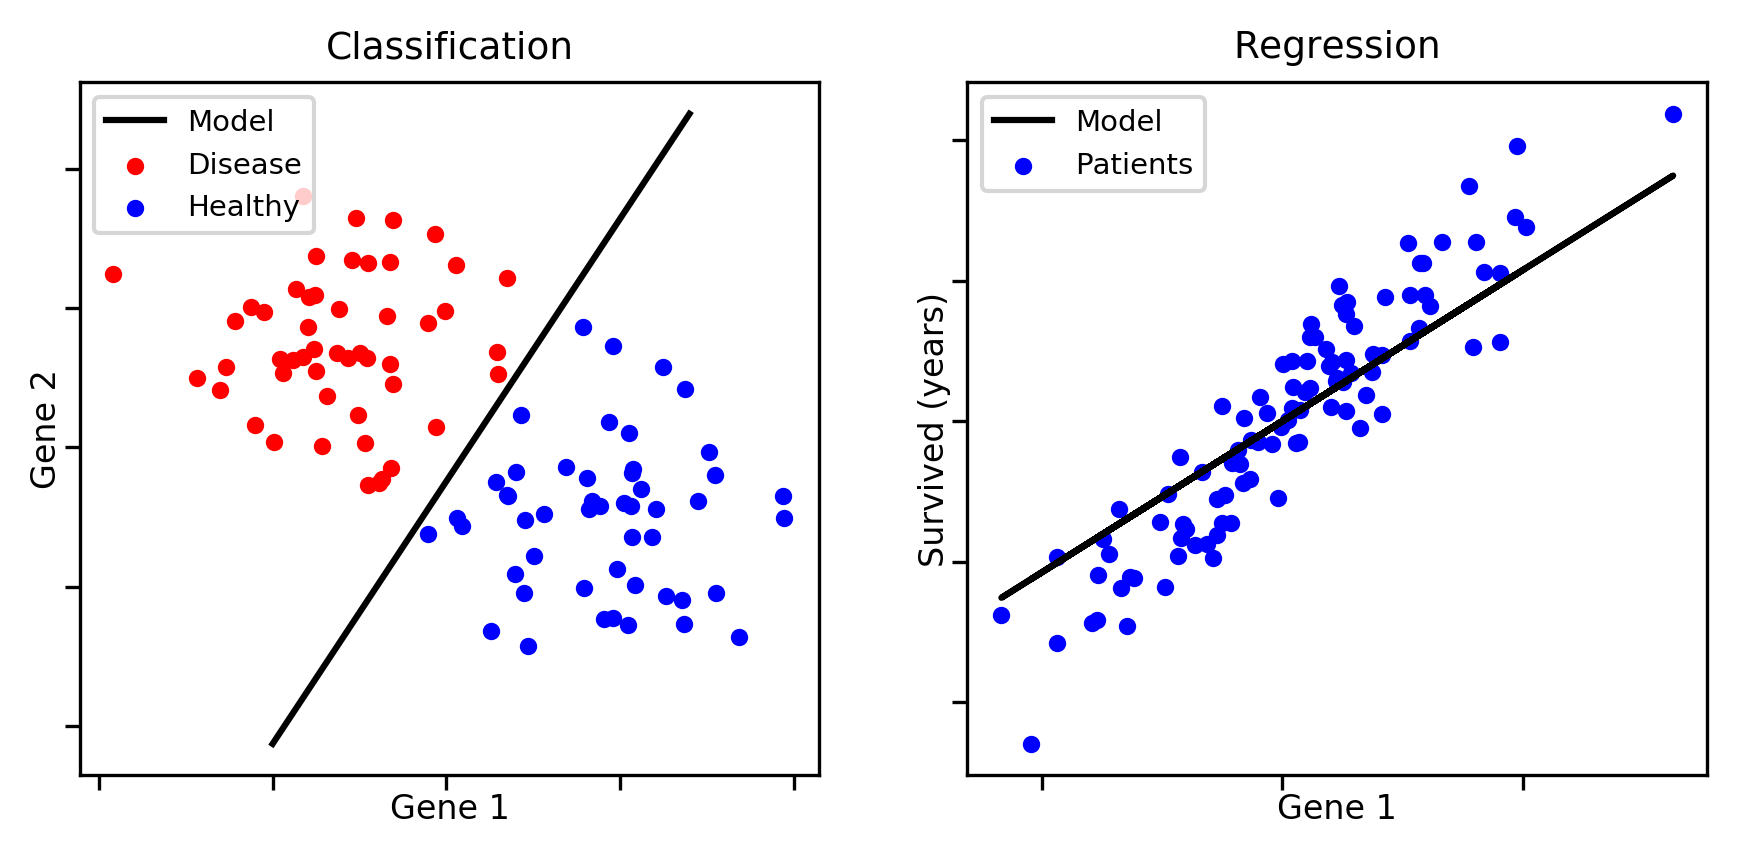
\includegraphics[width=\linewidth]{./imagenes/cr}
	\end{figure}
\end{frame}

\begin{frame}[fragile]{Clasificación no balanceada.}
	\begin{figure}[H]
	\centering
	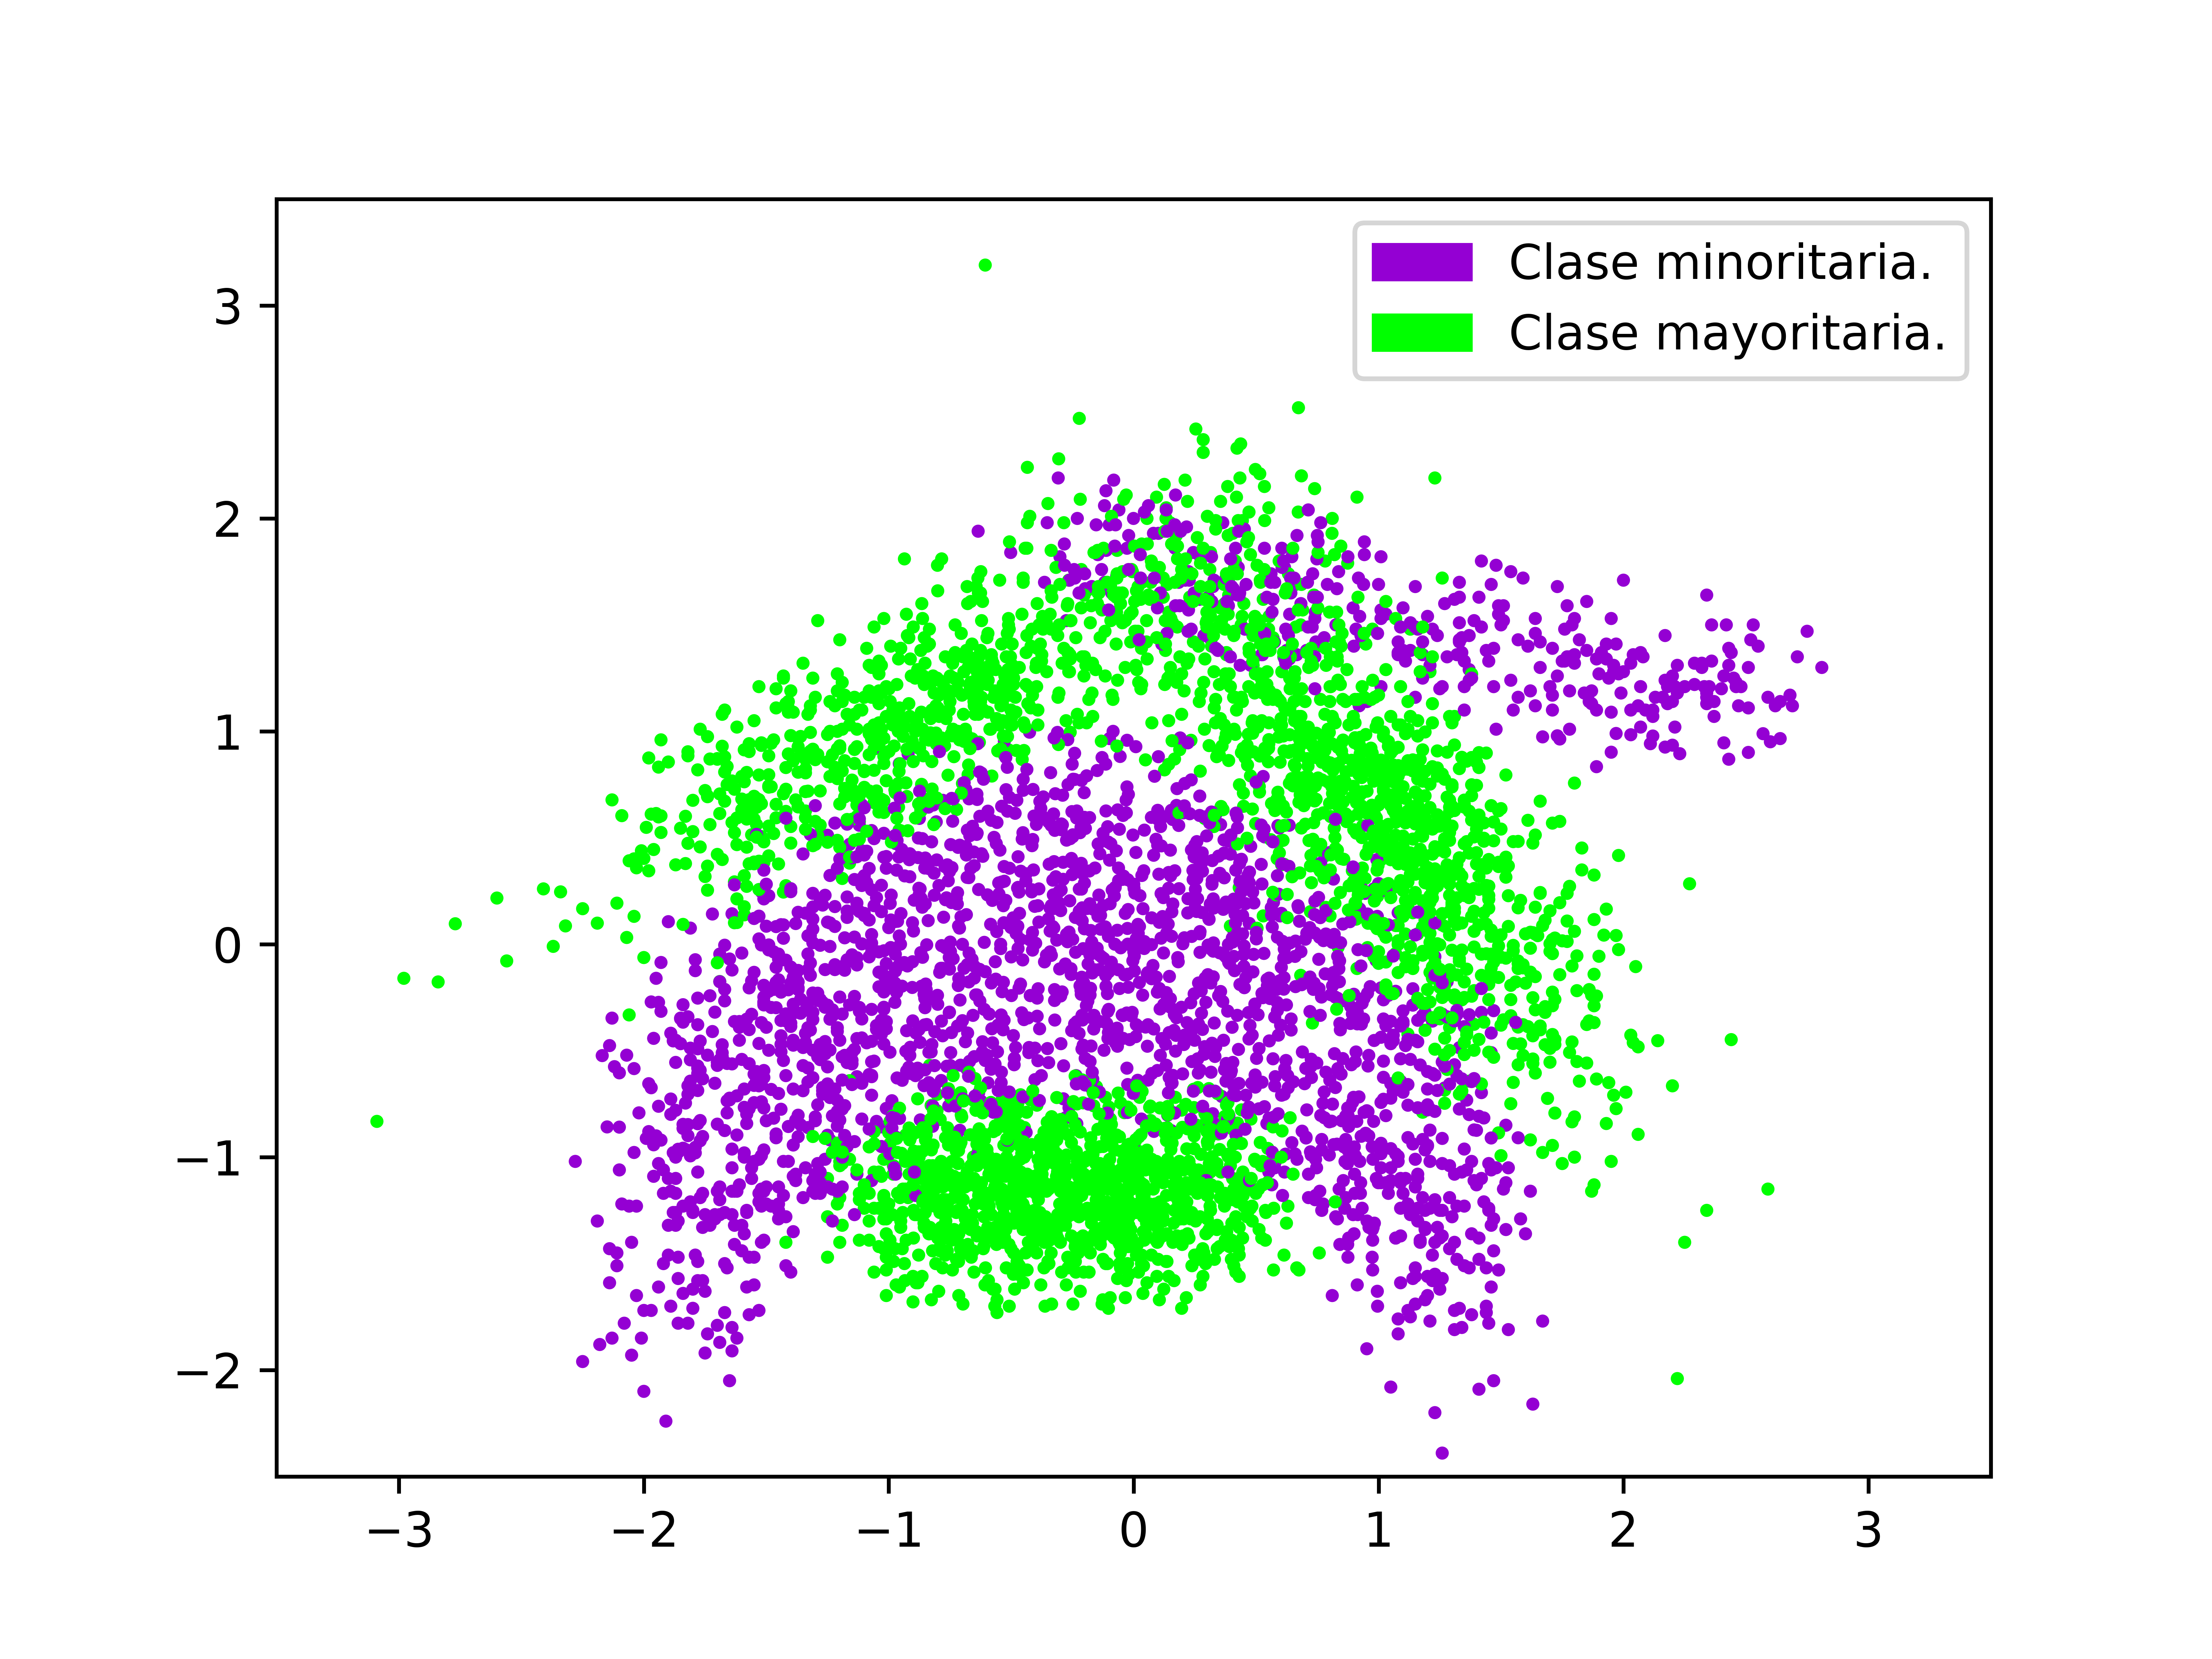
\includegraphics[width=\linewidth]{./imagenes/original}
	\end{figure}
\end{frame}

\begin{frame}[fragile]{Clasificación no balanceada.}
	\begin{figure}[H]
	\centering
	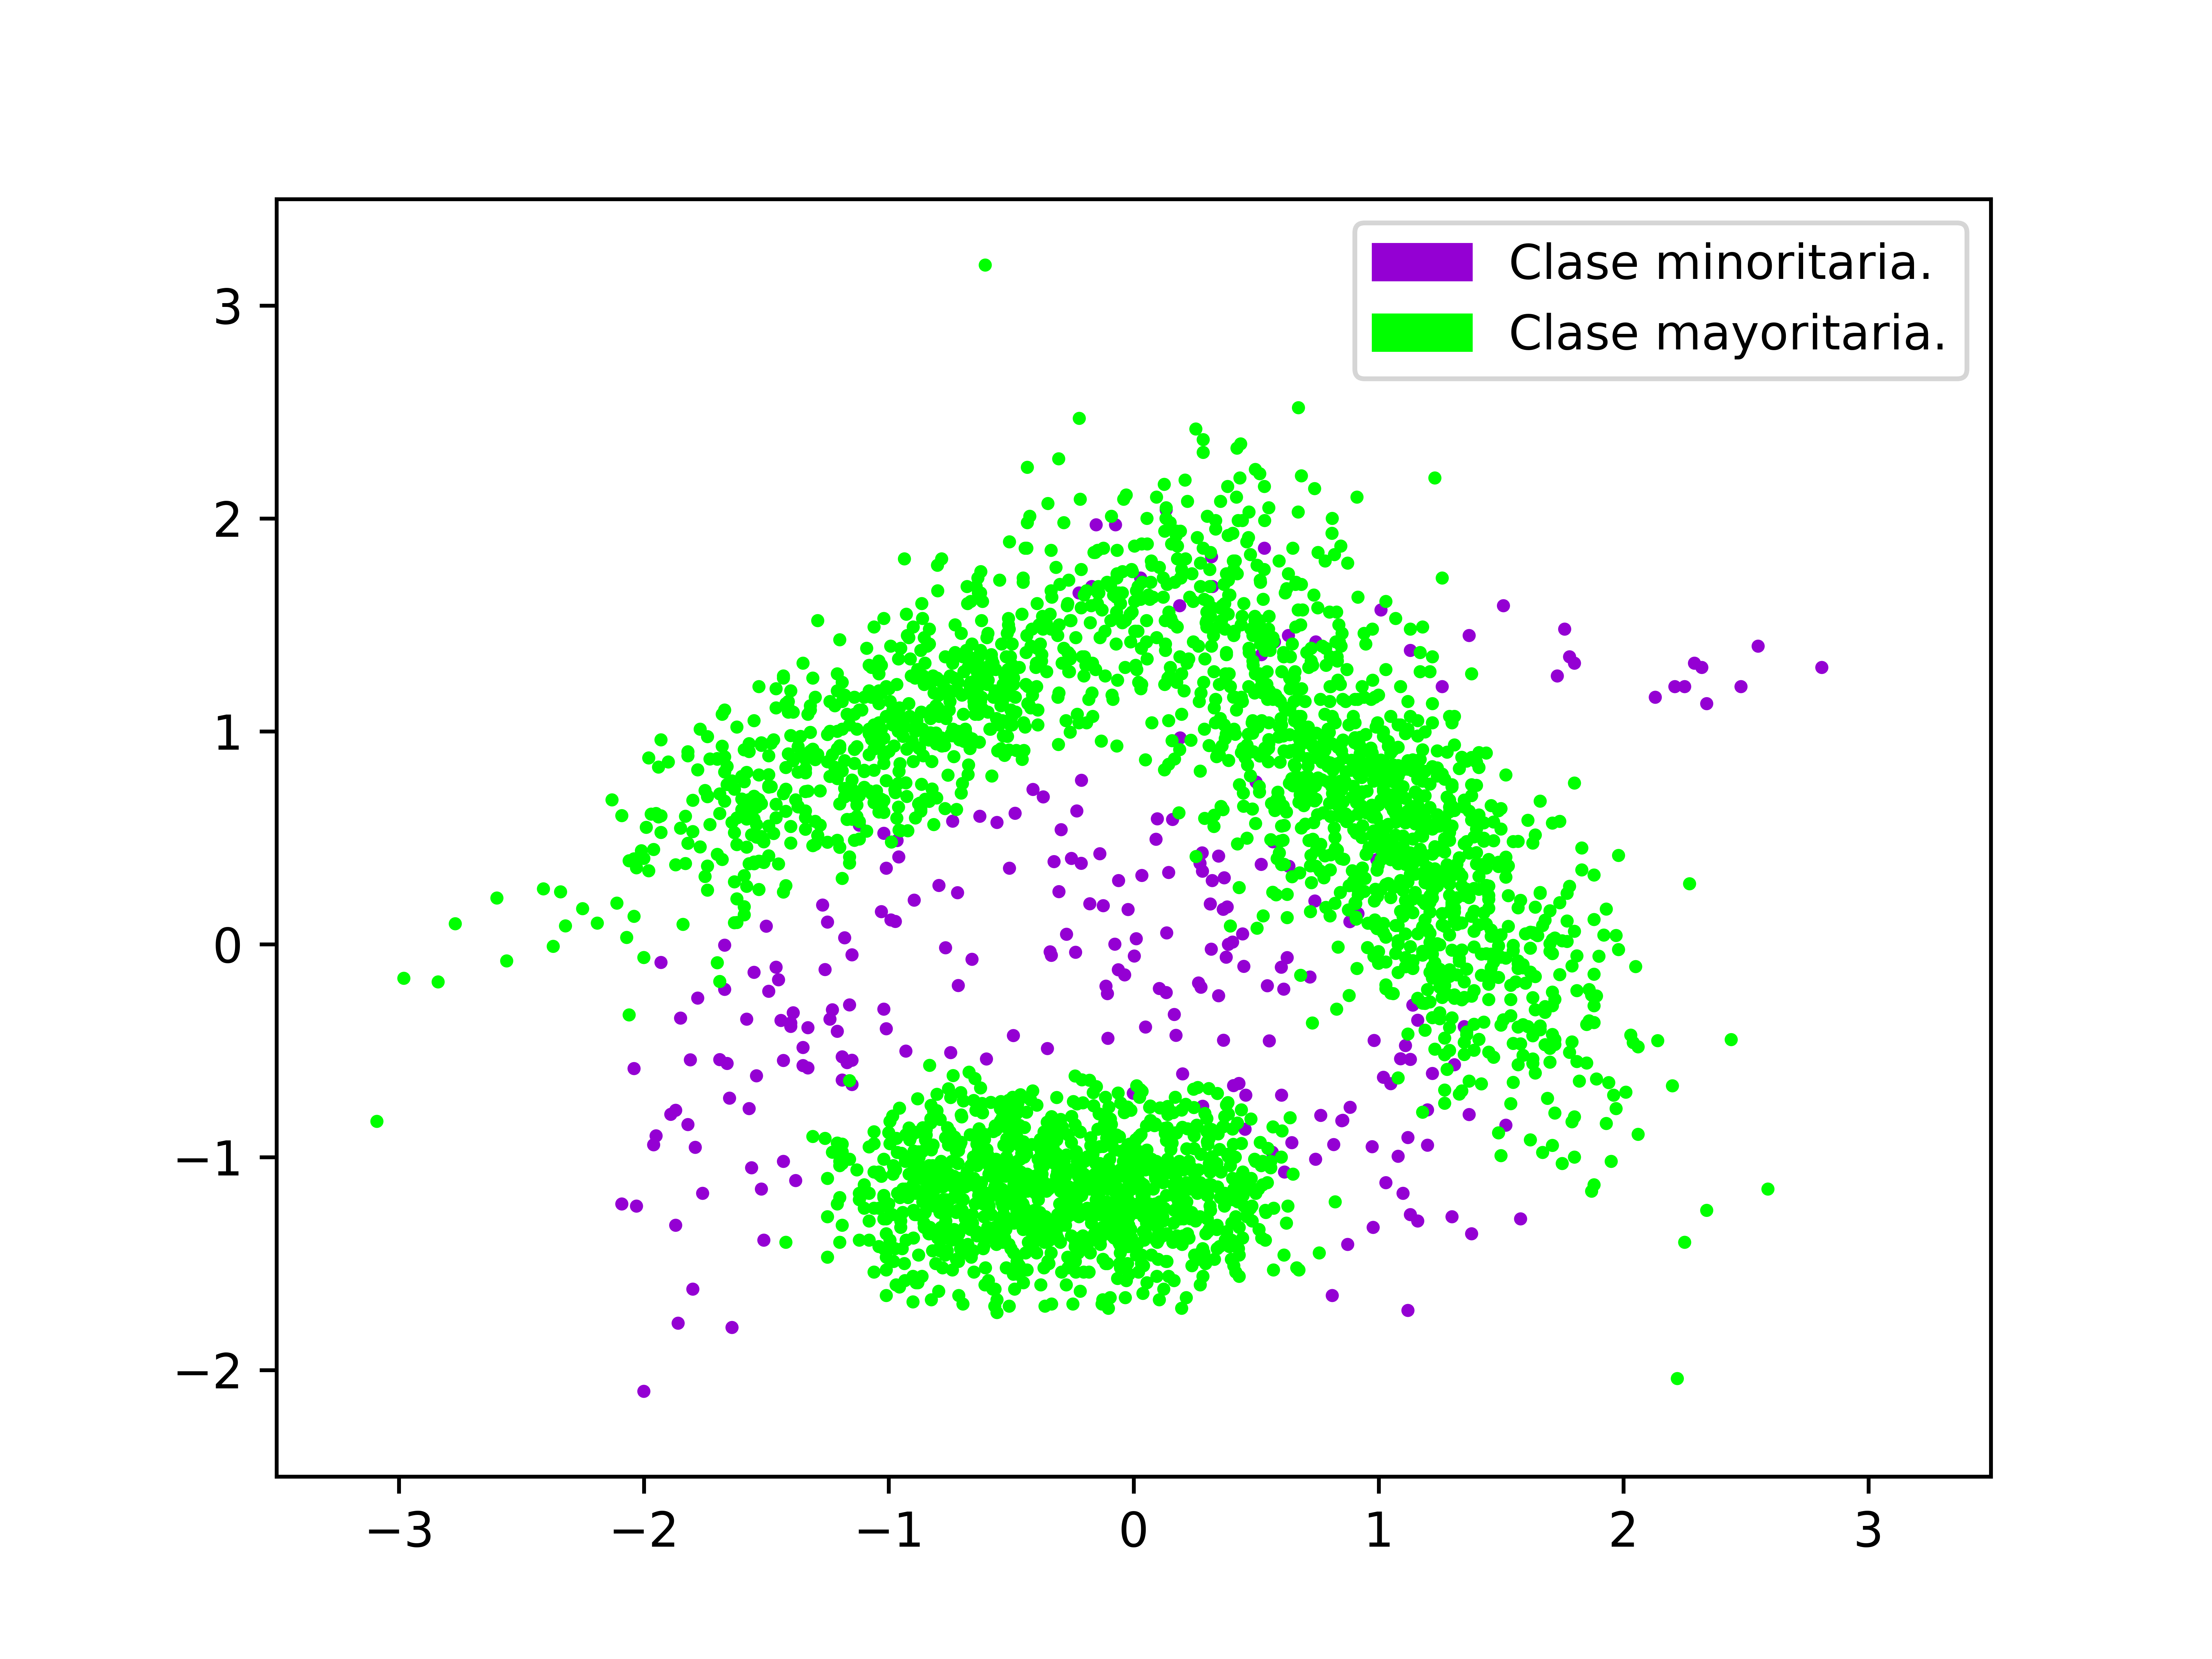
\includegraphics[width=\linewidth]{./imagenes/imbalanced}
	\end{figure}
\end{frame}

\section{Objetivos.}

\begin{frame}[fragile]{Objetivos.}
	\begin{itemize}
		\item Revisión bibliográfica del estado del arte.
		\item Estudio de requisitos y diseño de implementación.
		\item Implementación y prueba de los algoritmos.
		\item Comparación de los resultados obtenidos. 
	\end{itemize}
\end{frame}

\section{Planificación y diseño.}

\begin{frame}[fragile]{Planificación.}
	\begin{figure}
	\centering
    	\scalebox{.85}{\begin{ganttchart}[
canvas/.append style={fill=none, draw=black!5, line width=.75pt},
vgrid={*1{draw=black!5, line width=.75pt}},
today=20,
today label font=\scriptsize\scshape,
title/.style={draw=none, fill=none},
title label font=\scshape\footnotesize,
title label node/.append style={below=7pt},
include title in canvas=false,
bar/.append style={draw=none, fill=black!63}
]{1}{20}

\shorthandoff{"}
\gantttitlelist{"Sep", "Oct", "Nov", "Dic", "Ene", "Feb", "Mar", "Abr", "May", "Jun"}{2} \\
\shorthandon{"}
\ganttbar{Investigación}{1}{3} \\
\ganttbar{Análisis}{4}{5} \\
\ganttbar{Diseño}{6}{7} \\
\ganttbar{Implementación}{8}{17} \\
\ganttbar{Pruebas}{10}{17} \\
\ganttbar{Memoria}{16}{20}
\end{ganttchart}}
	\end{figure}
\end{frame}

\begin{frame}[fragile]{Diagrama de paquetes.}
	\begin{figure}[H]
	\centering
	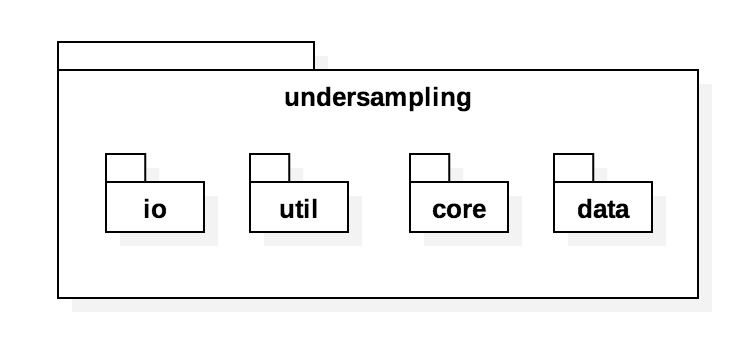
\includegraphics[width=\linewidth]{./imagenes/3_paquetes}
	\end{figure}
\end{frame}

\begin{frame}[fragile]{Diagrama de clases simplificado.}
	\begin{figure}[H]
	\centering
	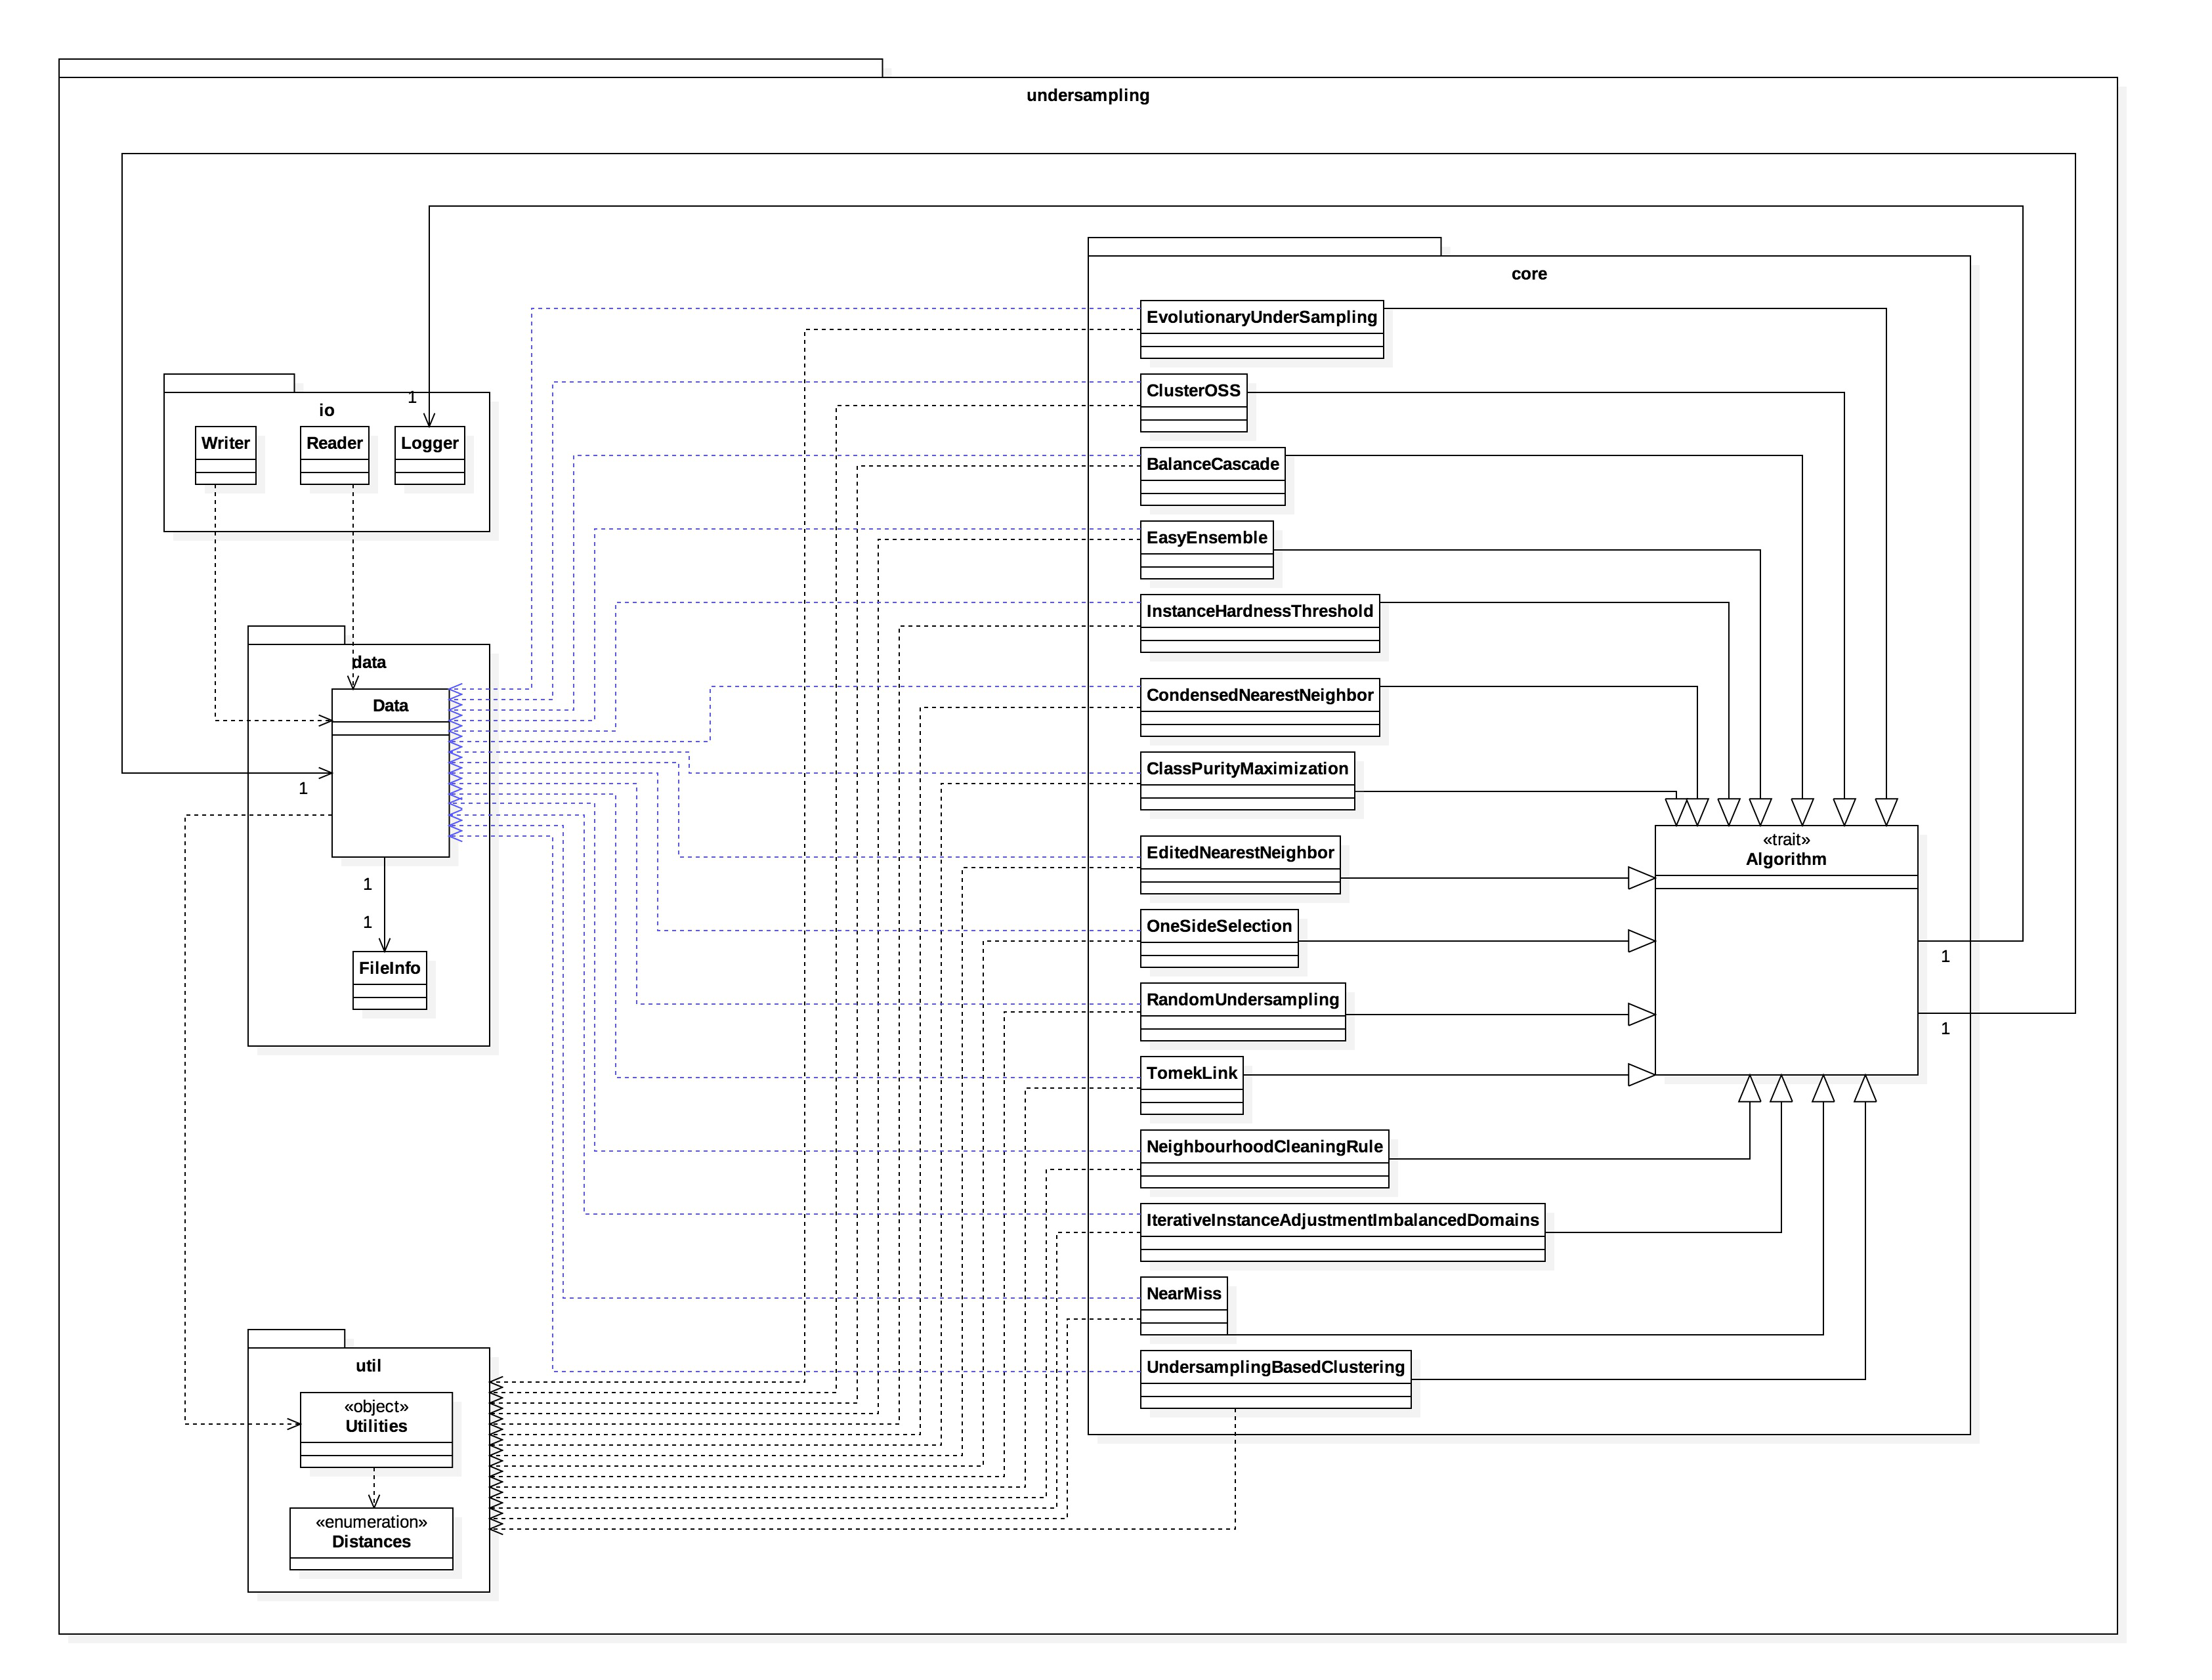
\includegraphics[scale=0.09]{./imagenes/3_clases_simplificado}
	\end{figure}
\end{frame}

\begin{frame}[fragile]{Requisitos funcionales.}
	\begin{itemize}
		\item Alta velocidad de procesamiento.
		\item Diferentes formatos de entrada.
		\item Diferentes formatos de salida.
		\item Seguro a errores.
		\item Datos intactos.
	\end{itemize}
\end{frame}

\section{Algoritmos seleccionados.}

\begin{frame}[fragile]{Balance Cascade.}
\textit{``Exploratory Undersampling for Class-Imbalance Learning} escrito por \textit{Xu-Ying Liu, Jianxin Wu y Zhi-Hua Zhou''} \cite{bc-ee} \\
\bigskip
\bigskip

Particiones $\rightarrow$ Clasificador $\rightarrow$ Combinar
\end{frame}

\begin{frame}[fragile]{Class Purity Maximization algorithm.}
\textit{``An Unsupervised Learning Approach to Resolving the Data Imbalanced Issue in Supervised Learning Problems in Functional Genomics} escrito por \textit{Kihoon Yoon y Stephen Kwek''} \cite{cpm} \\
\bigskip
\bigskip

Particiones en clústeres mientras obtengamos un conjunto más puro.
\end{frame}

\begin{frame}[fragile]{ClusterOSS.}
\textit{``ClusterOSS: a new undersampling method for imbalanced learning.''} escrito por \textit{Victor H Barella, Eduardo P Costa y André C. P. L. F. Carvalho} \cite{clusteross} \\
\bigskip
\bigskip

Clústeres $\rightarrow$ Elementos más representativos $\rightarrow$ Tomek Link
\end{frame}

\begin{frame}[fragile]{Condensed Nearest Neighbor decision rule.}
\textit{``The Condensed Nearest Neighbor Rule''} escrito por \textit{P. Hart} \cite{cnn} \\
\bigskip
\bigskip

Puntos innecesarios: se puede clasificar con el conjunto de puntos que tenemos actualmente.
\end{frame}

\begin{frame}[fragile]{Easy Ensemble.}
\textit{``Exploratory Undersampling for Class-Imbalance Learning''} escrito por \textit{Xu-Ying Liu, Jianxin Wu y Zhi-Hua Zhou} \cite{bc-ee} \\
\bigskip
\bigskip

Particiones $\rightarrow$ Clasificador $\rightarrow$ Combinar \\
Particiones $\rightarrow$ Combinar
\end{frame}

\begin{frame}[fragile]{Edited Nearest Neighbour rule.}
\textit{``Asymptotic Properties of Nearest Neighbor Rules Using Edited Data''} escrito por \textit{Dennis L. Wilson} \cite{enn} \\
\bigskip
\bigskip

Puntos redundantes: podemos predecir su clase usando todos los puntos del conjunto original menos el.
\end{frame}

\begin{frame}[fragile]{Evolutionary Undersampling.}
\textit{``Evolutionary Under-Sampling for Classification with Imbalanced Data Sets: Proposals y Taxonomy''} escrito por \textit{Salvador Garcia y Francisco Herrera} \cite{eus} \\
\bigskip
\bigskip

Vector de tamaño $\left | conjunto\_original \right |$ formado por unos y/o ceros: representa un subconjunto de elementos del conjunto original. Si en la posición \textit{i} del vector hay un uno, la instancia \textit{i} está incluida en dicho subconjunto.
\end{frame}

\begin{frame}[fragile]{Instance Hardness Threshold.}
\textit{``An Empirical Study of Instance Hardness''} escrito por \textit{Michael R. Smith, Tony Martinez y Christophe Giraud-Carrier} \cite{ihts} \\
\bigskip
\bigskip

Clasificar las instancias según su dureza: alta, baja o ninguna. Las instancias con una dureza alta se consideran que están mal clasificadas o son ruidosas $\rightarrow$ son eliminadas del conjunto de datos.
\end{frame}

\begin{frame}[fragile]{Iterative Instance Adjustment for Imbalanced Domains.}
\textit{``Addressing imbalanced classification with instance generation techniques: IPADE-ID''} escrito por \textit{Victoria López, Isaac Triguero, Cristóbal J. Carmona, Salvador García y Francisco Herrera} \cite{ipade} \\
\bigskip
\bigskip

Inicializar la población con las instancias más relevantes $\rightarrow$ Aplicamos de forma iterativa una versión simplificada del algoritmo \textit{Differential Evolution}.
\end{frame}

\begin{frame}[fragile]{NearMiss.}
\textit{``kNN Approach to Unbalanced Data Distribution: A Case Study involving Information Extraction''} escrito por \textit{Jianping Zhang y Inderjeet Mani} \cite{nm} \\
\bigskip
\bigskip

Eliminar los vecinos mayoritarios que sean redundantes:
\newline
\newline
NearMiss 1: Distancia media a sus tres vecinos de la clase minoritaria más cercanos sea menor. \\
NearMiss 2: Distancia media a sus tres vecinos de la clase minoritaria más lejanos sea menor. \\
NearMiss 3: Seleccionamos de forma aleatoria una cantidad de elementos mayoritarios para cada elemento minoritario.
\end{frame}

\begin{frame}[fragile]{Neighbourhood Cleaning Rule.}
\textit{``Improving Identification of Difficult Small Classes by Balancing Class Distribution''} escrito por \textit{J. Laurikkala} \cite{ncl} \\
\bigskip
\bigskip

Eliminar vecinos que clasifican de forma errónea otras instancias. \\
ENN $\rightarrow$ Predecir clase con los tres vecinos más cercanos $\rightarrow$ Incorrecta: eliminamos sus vecinos.
\end{frame}

\begin{frame}[fragile]{One-Side Selection.}
\textit{``Addressing the Curse of Imbalanced Training Sets: One-Side Selection''} escrito por \textit{Miroslav Kubat y Stan Matwin} \cite{oss} \\
\bigskip
\bigskip

Detectar ejemplos mal clasificados usando las instancias minoritarias y una mayoritaria al azar $\rightarrow$ Tomek Link: instancias minoritarias y las instancias mal clasificadas.
\end{frame}

\begin{frame}[fragile]{Random Undersampling.}
Eliminar instancias mayoritarias de forma aleatoria. \\
\end{frame}

\begin{frame}[fragile]{Tomek Link.}
\textit{``Two Modifications of CNN''} escrito por \textit{Ivan Tomek} \cite{tl} \\
\bigskip
\bigskip

Instancias ruidosas: vecino más cercano de la clase opuesta y si son el vecino más cercano entre sí, ambos elementos forman un \textit{tomek-link}
\end{frame}

\begin{frame}[fragile]{Undersampling Based on Clustering.}
\textit{``Under-Sampling Approaches for Improving Prediction of the Minority Class in an Imbalanced Dataset''} escrito por \textit{Show-Jane Yen y Yue-Shi Lee} \cite{sbc} \\
\bigskip
\bigskip

Conjunto de datos balanceado en cada \textit{clúster} y devolver la unión de todos los subconjuntos balanceados formado en cada \textit{clúster}
\end{frame}

\section{Scala.}

\begin{frame}[fragile]{Patrón de diseño mixto.}
	\begin{figure}[H]
	\centering
	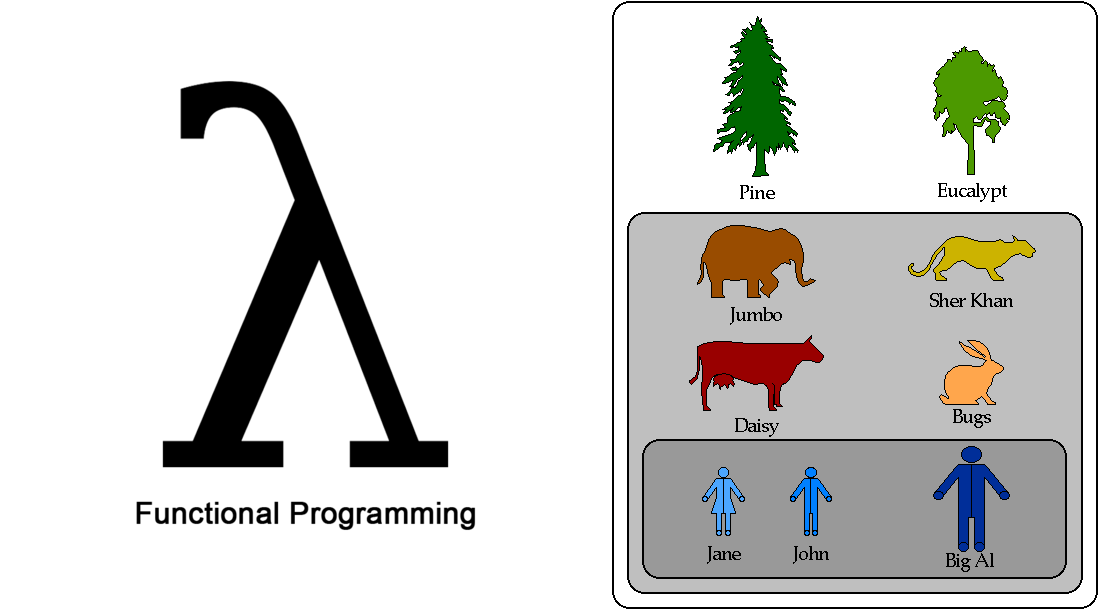
\includegraphics[width=\linewidth]{./imagenes/patron}
	\end{figure}
\end{frame}


\begin{frame}[fragile]{Simplicidad.}
\begin{lstlisting}[frame=single, basicstyle=\scriptsize, breaklines=true]
val r = new scala.util.Random
val d = (0 until 10).map(_ => (0 until 10).map(_ => r.nextDouble))
\end{lstlisting} 
\end{frame}

\begin{frame}[fragile]{Simplicidad.}
\begin{lstlisting}[frame=single, basicstyle=\scriptsize, breaklines=true]
public class Persona {
    private final String nombre;
    private final String apellido;
    public Person(String nombre, String apellido) {
        this.nombre = nombre;
        this.apellido = apellido;
    }
    public String getNombre() {
        return nombre;
    }
    public String getApellido() {
        return apellido;
    }
}
\end{lstlisting}
\end{frame}

\begin{frame}[fragile]{Simplicidad.}
\begin{lstlisting}[frame=single, basicstyle=\scriptsize, breaklines=true]
class Persona(val nombre: String, val apellido: String)
\end{lstlisting} 
\end{frame}

\begin{frame}[fragile]{Escalabilidad.}
	\begin{figure}[H]
	\centering
	
\includegraphics[scale=0.15]{./imagenes/scalable}
	\end{figure}
\end{frame}

\begin{frame}[fragile]{Modificadores de visibilidad.}
	\begin{itemize}
		\item Publico.
		\item Protegido: \textit{protected}.
		\item Privado: \textit{private}.
		\item Protegido[scope]: \textit{protected[scope]}.
		\item Privado[scope]: \textit{private[scope]}.
	\end{itemize}
\end{frame}

\begin{frame}[fragile]{Paralelismo.}
\begin{lstlisting}[frame=single, basicstyle=\scriptsize, breaklines=true]
scala> Array(0, 1, 2, 3, 4, 5).foreach(print)
res0: 012345
\end{lstlisting}

\begin{lstlisting}[frame=single, basicstyle=\scriptsize, breaklines=true]
scala> Array(0, 1, 2, 3, 4, 5).par.foreach(print)
res1: 035421
\end{lstlisting}
\end{frame}

\begin{frame}[fragile]{Ausencia de Scala.}
	\begin{figure}[H]
	\centering
	
\includegraphics[scale=0.1]{./imagenes/prohibited}
	\end{figure}
\end{frame}

\section{Descripción técnica.}

\begin{frame}[fragile]{Documentación.}
	\begin{center}
	\href{https://nestorrv.github.io}{https://nestorrv.github.io}
	\end{center}
	\vspace{-1cm}
	\begin{figure}[H]
	\centering
	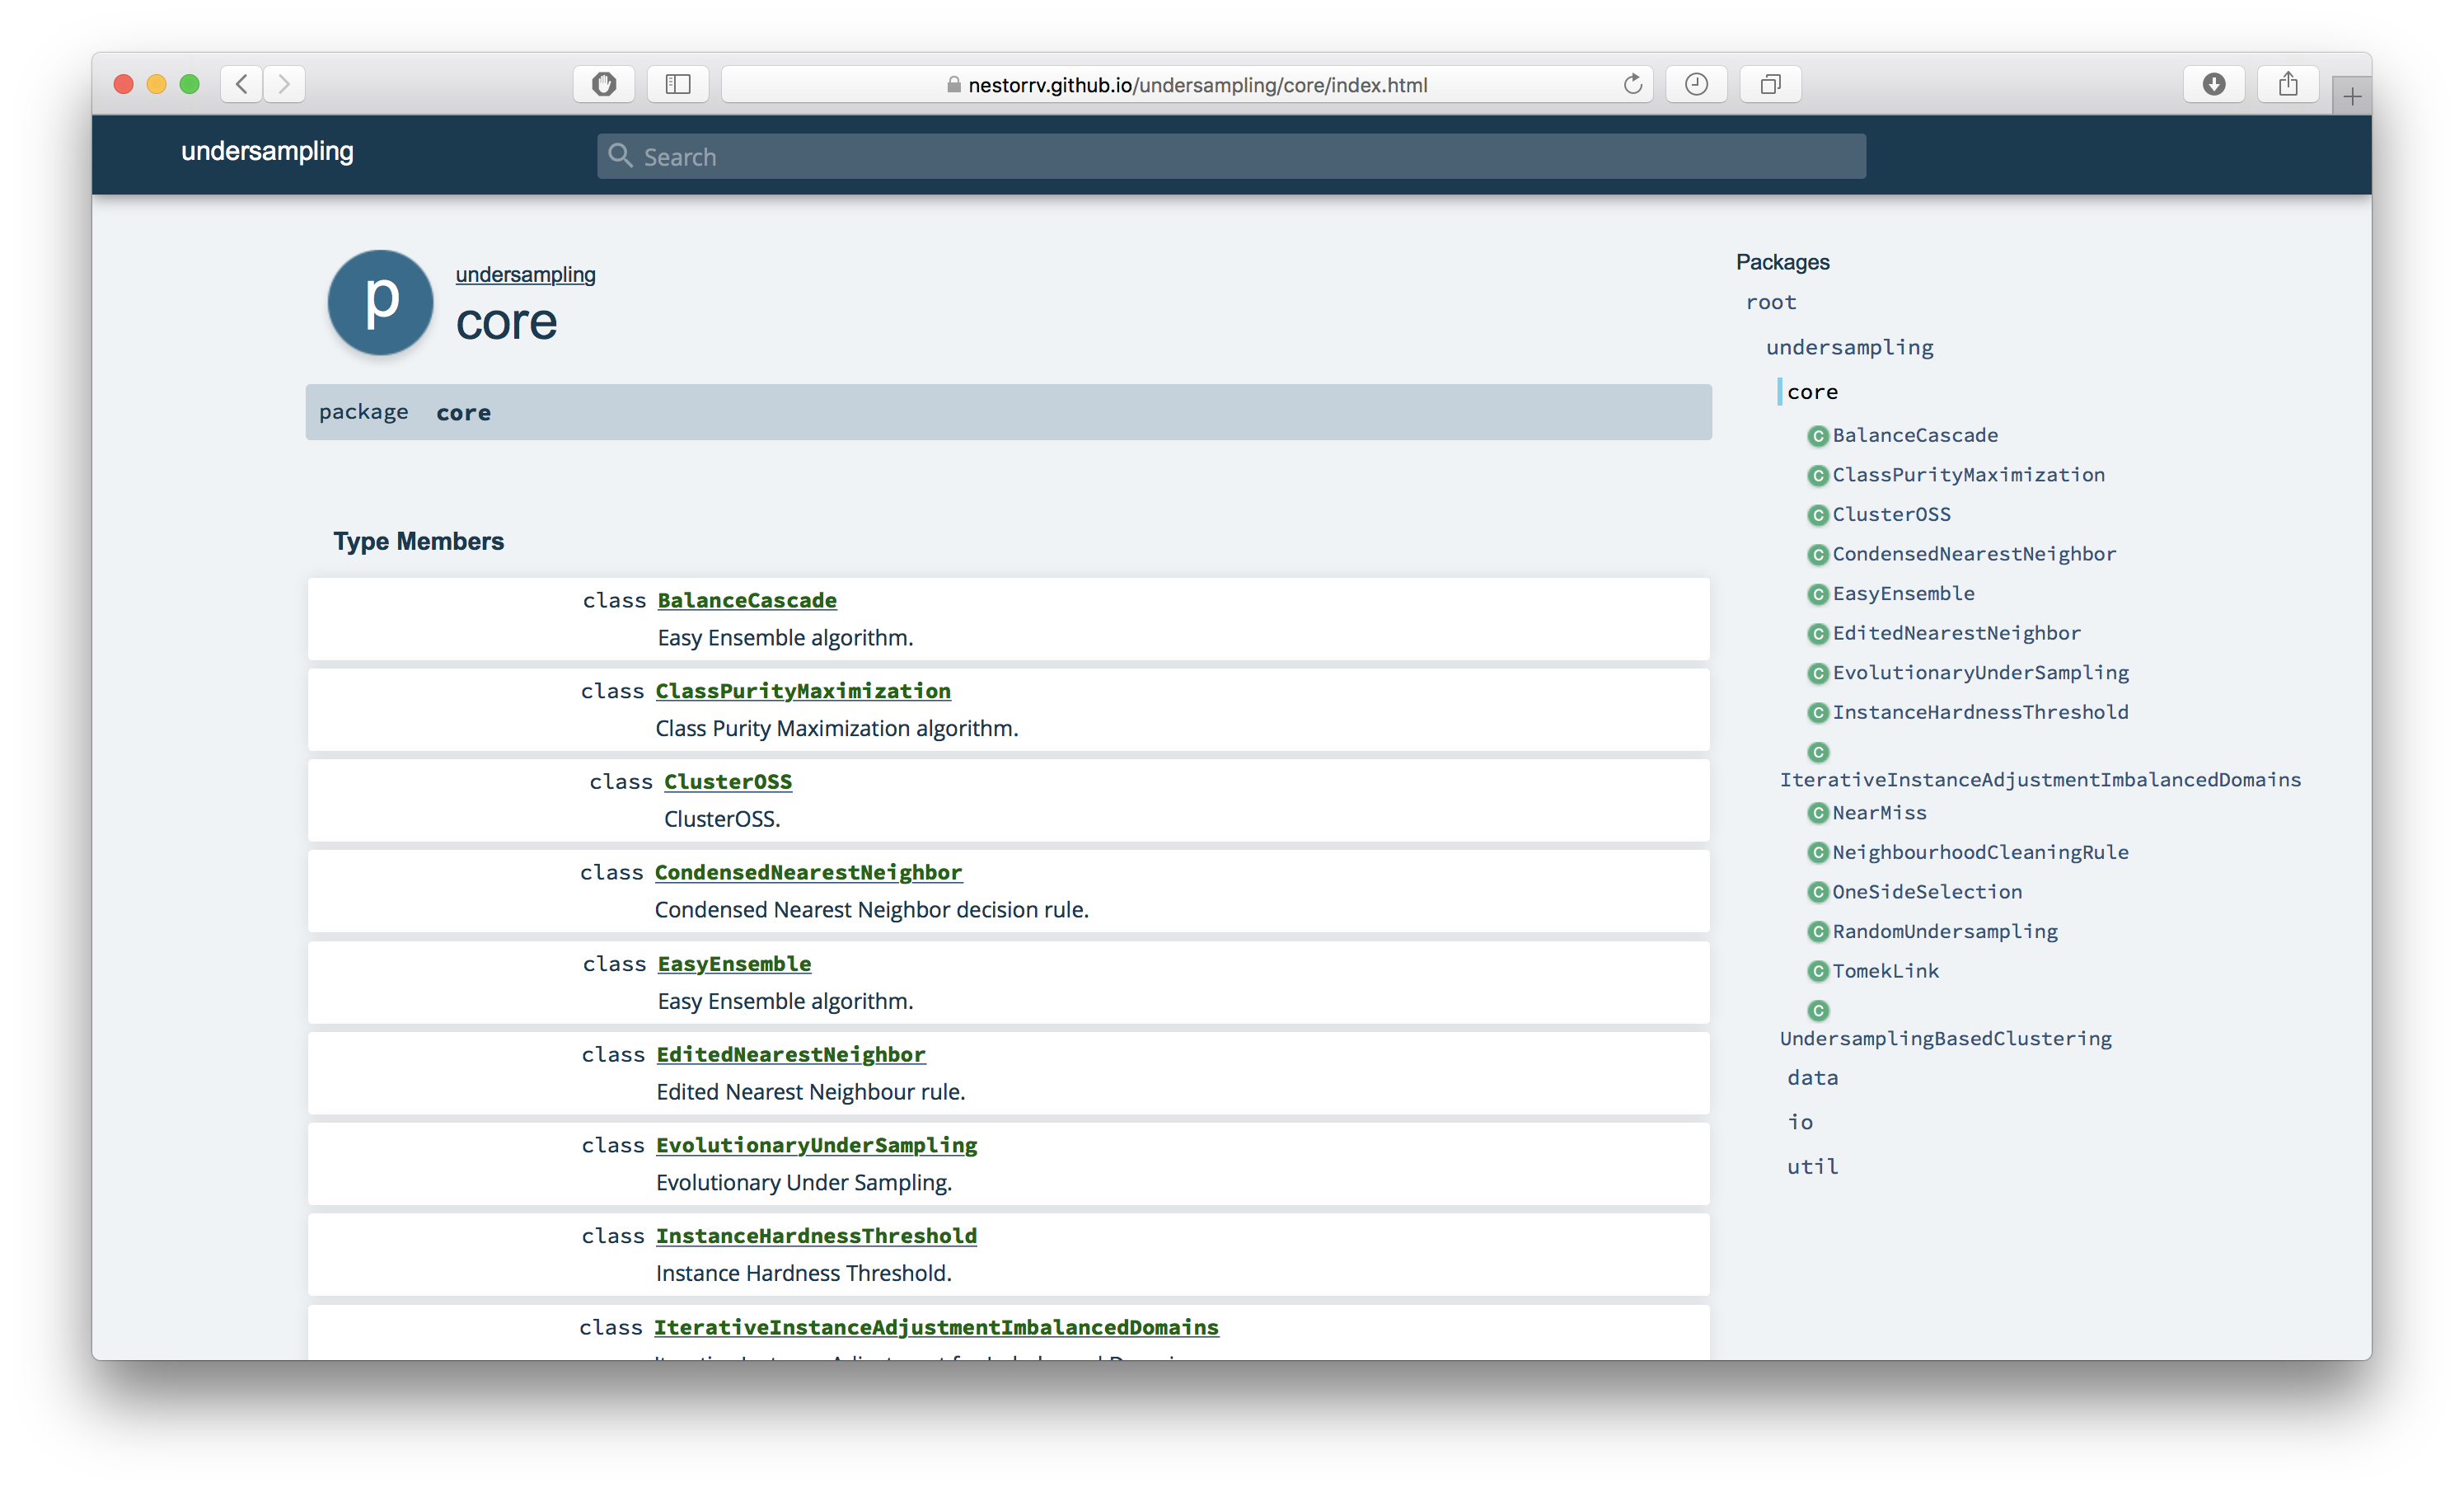
\includegraphics[scale=0.11]{./imagenes/doc}
	\end{figure}
\end{frame}

\begin{frame}[fragile]{sample.}
\begin{lstlisting}[frame=single, basicstyle=\scriptsize, breaklines=true]
sample(file: Option[String], ...)
\end{lstlisting}
\end{frame}

\begin{frame}[fragile]{Manual de usuario.}
\begin{lstlisting}[frame=single, basicstyle=\scriptsize, breaklines=true]
import undersampling.io.Reader
import undersampling.core.NeighbourhoodCleaningRule
import undersampling.io.Writer

val reader = new Reader
val writer = new Writer

val csvData = reader.readDelimitedText(file = pathToFile)
val arffData = reader.readArff(file = pathToFile)

val nclCSV = new NeighbourhoodCleaningRule(csvData, seed = 0L)
val resultCSV = nclCSV.sample(file = Option("milogCSV.log"))

val nclARFF = new NeighbourhoodCleaningRule(arffData, seed = 0L)
val resultARFF = nclARFF.sample(file = Option("milogARFF.log"))

writer.writeDelimitedText(file = "salidaCSV.csv", data = resultCSV)
writer.writeArff(file = "salidaARFF.arff", data = resultARFF)
\end{lstlisting}
\end{frame}

\section{Experimentación.}

\begin{frame}{Porcentaje de reducción.}
\scalebox{0.45}{\begin{tabular}{l|ccccccccccccccc|c}
\textbf{Dataset} & \textbf{BC} & \textbf{ClusterOSS} & \textbf{CNN} & \textbf{CPM} & \textbf{EE} & \textbf{ENN} & \textbf{EUS} & \textbf{IHTS} & \textbf{IPADE} & \textbf{NCL} & \textbf{NM} & \textbf{OSS} & \textbf{RU} & \textbf{SBC} & \textbf{TL} & \textbf{Media} \\
\midrule
\textbf{ecoli-0\_vs\_1} & \cellcolor[rgb]{ .988,  .988,  1}30 & \cellcolor[rgb]{ .98,  .612,  .62}70.91 & \cellcolor[rgb]{ .973,  .412,  .42}92.27 & \cellcolor[rgb]{ .976,  .42,  .427}91.82 & \cellcolor[rgb]{ .988,  .988,  1}30 & \cellcolor[rgb]{ .353,  .541,  .776}0 & \cellcolor[rgb]{ .988,  .988,  1}30 & \cellcolor[rgb]{ .984,  .788,  .8}51.82 & \cellcolor[rgb]{ .976,  .424,  .431}91.36 & \cellcolor[rgb]{ .447,  .608,  .808}4.55 & \cellcolor[rgb]{ .988,  .988,  1}30 & \cellcolor[rgb]{ .988,  .878,  .886}42.27 & \cellcolor[rgb]{ .988,  .988,  1}30 & \cellcolor[rgb]{ .439,  .6,  .804}4.09 & \cellcolor[rgb]{ .447,  .608,  .808}4.55 & 40.24 \\
\textbf{ecoli1} & \cellcolor[rgb]{ .988,  .988,  1}54.17 & \cellcolor[rgb]{ .976,  .506,  .518}83.33 & \cellcolor[rgb]{ .98,  .627,  .635}76.19 & \cellcolor[rgb]{ .98,  .651,  .659}74.7 & \cellcolor[rgb]{ .988,  .988,  1}54.17 & \cellcolor[rgb]{ .353,  .541,  .776}4.46 & \cellcolor[rgb]{ .988,  .988,  1}54.17 & \cellcolor[rgb]{ .98,  .667,  .675}73.81 & \cellcolor[rgb]{ .973,  .412,  .42}88.99 & \cellcolor[rgb]{ .435,  .6,  .804}11.01 & \cellcolor[rgb]{ .988,  .988,  1}54.17 & \cellcolor[rgb]{ .714,  .792,  .902}32.74 & \cellcolor[rgb]{ .988,  .988,  1}54.17 & \cellcolor[rgb]{ .467,  .62,  .816}13.39 & \cellcolor[rgb]{ .447,  .608,  .808}11.9 & 49.42 \\
\textbf{ecoli2} & \cellcolor[rgb]{ .988,  .988,  1}69.05 & \cellcolor[rgb]{ .976,  .486,  .494}89.88 & \cellcolor[rgb]{ .984,  .725,  .733}80.06 & \cellcolor[rgb]{ .98,  .694,  .706}81.25 & \cellcolor[rgb]{ .988,  .988,  1}69.05 & \cellcolor[rgb]{ .353,  .541,  .776}2.08 & \cellcolor[rgb]{ .988,  .988,  1}69.05 & \cellcolor[rgb]{ .98,  .694,  .706}81.25 & \cellcolor[rgb]{ .973,  .412,  .42}92.86 & \cellcolor[rgb]{ .384,  .565,  .788}5.65 & \cellcolor[rgb]{ .988,  .988,  1}69.05 & \cellcolor[rgb]{ .486,  .635,  .824}16.37 & \cellcolor[rgb]{ .988,  .988,  1}69.05 & \cellcolor[rgb]{ .408,  .58,  .796}8.04 & \cellcolor[rgb]{ .4,  .573,  .792}7.14 & 53.99 \\
\textbf{ecoli3} & \cellcolor[rgb]{ .988,  .988,  1}79.17 & \cellcolor[rgb]{ .976,  .553,  .565}87.5 & \cellcolor[rgb]{ .988,  .898,  .91}80.95 & \cellcolor[rgb]{ .98,  .678,  .69}85.12 & \cellcolor[rgb]{ .988,  .988,  1}79.17 & \cellcolor[rgb]{ .353,  .541,  .776}3.57 & \cellcolor[rgb]{ .988,  .988,  1}79.17 & \cellcolor[rgb]{ .98,  .631,  .643}86.01 & \cellcolor[rgb]{ .973,  .412,  .42}90.18 & \cellcolor[rgb]{ .376,  .557,  .784}6.55 & \cellcolor[rgb]{ .988,  .988,  1}79.17 & \cellcolor[rgb]{ .537,  .671,  .839}25.6 & \cellcolor[rgb]{ .988,  .988,  1}79.17 & \cellcolor[rgb]{ .404,  .576,  .792}9.82 & \cellcolor[rgb]{ .384,  .565,  .788}7.74 & 58.59 \\
\textbf{glass-0-1-2-3\_vs\_4-5-6} & \cellcolor[rgb]{ .988,  .988,  1}52.34 & \cellcolor[rgb]{ .976,  .427,  .439}85.98 & \cellcolor[rgb]{ .976,  .435,  .447}85.51 & \cellcolor[rgb]{ .973,  .412,  .42}86.92 & \cellcolor[rgb]{ .988,  .988,  1}52.34 & \cellcolor[rgb]{ .353,  .541,  .776}3.74 & \cellcolor[rgb]{ .988,  .988,  1}52.34 & \cellcolor[rgb]{ .98,  .631,  .643}73.83 & \cellcolor[rgb]{ .976,  .435,  .447}85.51 & \cellcolor[rgb]{ .412,  .58,  .796}8.41 & \cellcolor[rgb]{ .988,  .988,  1}52.34 & \cellcolor[rgb]{ .412,  .58,  .796}8.41 & \cellcolor[rgb]{ .988,  .988,  1}52.34 & \cellcolor[rgb]{ .376,  .557,  .784}5.61 & \cellcolor[rgb]{ .376,  .557,  .784}5.61 & 47.41 \\
\textbf{glass0} & \cellcolor[rgb]{ .988,  .988,  1}34.58 & \cellcolor[rgb]{ .976,  .431,  .439}80.84 & \cellcolor[rgb]{ .98,  .639,  .651}63.55 & \cellcolor[rgb]{ .98,  .604,  .616}66.36 & \cellcolor[rgb]{ .988,  .988,  1}34.58 & \cellcolor[rgb]{ .353,  .541,  .776}14.49 & \cellcolor[rgb]{ .988,  .988,  1}34.58 & \cellcolor[rgb]{ .984,  .753,  .765}54.21 & \cellcolor[rgb]{ .973,  .412,  .42}82.24 & \cellcolor[rgb]{ .529,  .663,  .835}20.09 & \cellcolor[rgb]{ .988,  .988,  1}34.58 & \cellcolor[rgb]{ .988,  .957,  .969}37.38 & \cellcolor[rgb]{ .988,  .988,  1}34.58 & \cellcolor[rgb]{ .439,  .6,  .804}17.29 & \cellcolor[rgb]{ .541,  .675,  .843}20.56 & 41.99 \\
\textbf{glass1} & \cellcolor[rgb]{ .988,  .988,  1}28.97 & \cellcolor[rgb]{ .973,  .412,  .42}84.11 & \cellcolor[rgb]{ .98,  .675,  .682}59.35 & \cellcolor[rgb]{ .98,  .643,  .651}62.15 & \cellcolor[rgb]{ .988,  .988,  1}28.97 & \cellcolor[rgb]{ .353,  .541,  .776}10.28 & \cellcolor[rgb]{ .988,  .988,  1}28.97 & \cellcolor[rgb]{ .984,  .808,  .82}46.26 & \cellcolor[rgb]{ .976,  .443,  .451}81.31 & \cellcolor[rgb]{ .686,  .773,  .89}20.09 & \cellcolor[rgb]{ .988,  .988,  1}28.97 & \cellcolor[rgb]{ .812,  .863,  .937}23.83 & \cellcolor[rgb]{ .988,  .988,  1}28.97 & \cellcolor[rgb]{ .463,  .616,  .812}13.55 & \cellcolor[rgb]{ .671,  .765,  .886}19.63 & 37.69 \\
\textbf{glass6} & \cellcolor[rgb]{ .988,  .988,  1}72.9 & \cellcolor[rgb]{ .98,  .667,  .675}83.18 & \cellcolor[rgb]{ .973,  .412,  .42}91.12 & \cellcolor[rgb]{ .976,  .459,  .467}89.72 & \cellcolor[rgb]{ .988,  .988,  1}72.9 & \cellcolor[rgb]{ .353,  .541,  .776}0.47 & \cellcolor[rgb]{ .988,  .988,  1}72.9 & \cellcolor[rgb]{ .98,  .635,  .643}84.11 & \cellcolor[rgb]{ .976,  .518,  .525}87.85 & \cellcolor[rgb]{ .412,  .584,  .796}7.48 & \cellcolor[rgb]{ .988,  .988,  1}72.9 & \cellcolor[rgb]{ .867,  .902,  .957}59.35 & \cellcolor[rgb]{ .988,  .988,  1}72.9 & \cellcolor[rgb]{ .396,  .573,  .792}5.61 & \cellcolor[rgb]{ .396,  .573,  .792}5.61 & 58.6 \\
\textbf{haberman} & \cellcolor[rgb]{ .988,  .988,  1}47.06 & \cellcolor[rgb]{ .976,  .494,  .502}82.03 & \cellcolor[rgb]{ .98,  .98,  .996}46.73 & \cellcolor[rgb]{ .988,  .922,  .933}51.96 & \cellcolor[rgb]{ .988,  .988,  1}47.06 & \cellcolor[rgb]{ .353,  .541,  .776}10.78 & \cellcolor[rgb]{ .98,  .98,  .996}46.73 & \cellcolor[rgb]{ .98,  .62,  .627}73.2 & \cellcolor[rgb]{ .973,  .412,  .42}87.58 & \cellcolor[rgb]{ .569,  .694,  .851}23.2 & \cellcolor[rgb]{ .988,  .988,  1}47.06 & \cellcolor[rgb]{ .765,  .827,  .918}34.31 & \cellcolor[rgb]{ .988,  .988,  1}47.06 & \cellcolor[rgb]{ .718,  .796,  .902}31.7 & \cellcolor[rgb]{ .702,  .784,  .898}30.72 & 47.15 \\
\textbf{iris0} & \cellcolor[rgb]{ .988,  .988,  1}33.33 & \cellcolor[rgb]{ .976,  .478,  .486}91.33 & \cellcolor[rgb]{ .973,  .412,  .42}98.67 & \cellcolor[rgb]{ .973,  .412,  .42}98.67 & \cellcolor[rgb]{ .988,  .988,  1}33.33 & \cellcolor[rgb]{ .353,  .541,  .776}0 & \cellcolor[rgb]{ .988,  .988,  1}33.33 & \cellcolor[rgb]{ .984,  .8,  .812}54.67 & \cellcolor[rgb]{ .976,  .478,  .486}91.33 & \cellcolor[rgb]{ .353,  .541,  .776}0 & \cellcolor[rgb]{ .988,  .988,  1}33.33 & \cellcolor[rgb]{ .98,  .69,  .698}67.33 & \cellcolor[rgb]{ .988,  .988,  1}33.33 & \cellcolor[rgb]{ .376,  .557,  .784}1.33 & \cellcolor[rgb]{ .4,  .576,  .792}2.67 & 44.84 \\
\textbf{new-thyroid1} & \cellcolor[rgb]{ .988,  .988,  1}67.44 & \cellcolor[rgb]{ .984,  .706,  .718}80.93 & \cellcolor[rgb]{ .973,  .412,  .42}94.88 & \cellcolor[rgb]{ .976,  .431,  .443}93.95 & \cellcolor[rgb]{ .988,  .988,  1}67.44 & \cellcolor[rgb]{ .353,  .541,  .776}0.93 & \cellcolor[rgb]{ .988,  .988,  1}67.44 & \cellcolor[rgb]{ .988,  .973,  .98}68.37 & \cellcolor[rgb]{ .976,  .541,  .549}88.84 & \cellcolor[rgb]{ .4,  .573,  .792}6.05 & \cellcolor[rgb]{ .988,  .988,  1}67.44 & \cellcolor[rgb]{ .988,  .902,  .914}71.63 & \cellcolor[rgb]{ .988,  .988,  1}67.44 & \cellcolor[rgb]{ .373,  .553,  .78}3.26 & \cellcolor[rgb]{ .388,  .565,  .788}4.65 & 56.71 \\
\textbf{new-thyroid2} & \cellcolor[rgb]{ .988,  .988,  1}67.44 & \cellcolor[rgb]{ .98,  .635,  .643}83.26 & \cellcolor[rgb]{ .973,  .412,  .42}93.02 & \cellcolor[rgb]{ .976,  .424,  .431}92.56 & \cellcolor[rgb]{ .988,  .988,  1}67.44 & \cellcolor[rgb]{ .353,  .541,  .776}0.93 & \cellcolor[rgb]{ .988,  .988,  1}67.44 & \cellcolor[rgb]{ .98,  .675,  .686}81.4 & \cellcolor[rgb]{ .976,  .498,  .506}89.3 & \cellcolor[rgb]{ .396,  .569,  .788}5.58 & \cellcolor[rgb]{ .988,  .988,  1}67.44 & \cellcolor[rgb]{ .882,  .914,  .961}56.74 & \cellcolor[rgb]{ .988,  .988,  1}67.44 & \cellcolor[rgb]{ .38,  .561,  .784}4.19 & \cellcolor[rgb]{ .388,  .565,  .788}4.65 & 56.59 \\
\textbf{page-blocks0} & \cellcolor[rgb]{ .988,  .988,  1}79.57 & \cellcolor[rgb]{ .98,  .627,  .639}90.83 & \cellcolor[rgb]{ .98,  .635,  .647}90.61 & \cellcolor[rgb]{ .98,  .635,  .647}90.61 & \cellcolor[rgb]{ .988,  .988,  1}79.57 & \cellcolor[rgb]{ .353,  .541,  .776}1.13 & \cellcolor[rgb]{ .988,  .988,  1}79.59 & \cellcolor[rgb]{ .984,  .725,  .733}87.85 & \cellcolor[rgb]{ .973,  .412,  .42}97.53 & \cellcolor[rgb]{ .373,  .557,  .784}3.97 & \cellcolor[rgb]{ .988,  .988,  1}79.57 & \cellcolor[rgb]{ .471,  .624,  .816}15.97 & \cellcolor[rgb]{ .988,  .988,  1}79.57 & \cellcolor[rgb]{ .663,  .757,  .882}39.47 & \cellcolor[rgb]{ .384,  .561,  .784}5.23 & 61.4 \\
\textbf{pima} & \cellcolor[rgb]{ .988,  .988,  1}30.21 & \cellcolor[rgb]{ .976,  .541,  .549}79.04 & \cellcolor[rgb]{ .984,  .8,  .812}50.91 & \cellcolor[rgb]{ .984,  .796,  .808}51.3 & \cellcolor[rgb]{ .988,  .988,  1}30.21 & \cellcolor[rgb]{ .353,  .541,  .776}11.72 & \cellcolor[rgb]{ .988,  .988,  1}30.34 & \cellcolor[rgb]{ .98,  .69,  .702}62.63 & \cellcolor[rgb]{ .973,  .412,  .42}92.84 & \cellcolor[rgb]{ .788,  .847,  .929}24.48 & \cellcolor[rgb]{ .988,  .988,  1}30.21 & \cellcolor[rgb]{ .976,  .98,  .996}29.95 & \cellcolor[rgb]{ .988,  .988,  1}30.21 & \cellcolor[rgb]{ .988,  .988,  1}30.21 & \cellcolor[rgb]{ .886,  .918,  .965}27.34 & 40.77 \\
\textbf{segment0} & \cellcolor[rgb]{ .988,  .988,  1}71.49 & \cellcolor[rgb]{ .98,  .647,  .655}87.56 & \cellcolor[rgb]{ .976,  .443,  .451}97.01 & \cellcolor[rgb]{ .976,  .439,  .447}97.18 & \cellcolor[rgb]{ .988,  .988,  1}71.49 & \cellcolor[rgb]{ .353,  .541,  .776}0.78 & \cellcolor[rgb]{ .988,  .984,  .996}71.75 & \cellcolor[rgb]{ .961,  .969,  .988}68.59 & \cellcolor[rgb]{ .973,  .412,  .42}98.35 & \cellcolor[rgb]{ .357,  .541,  .776}1.34 & \cellcolor[rgb]{ .988,  .988,  1}71.49 & \cellcolor[rgb]{ .525,  .663,  .835}20.23 & \cellcolor[rgb]{ .988,  .988,  1}71.49 & \cellcolor[rgb]{ .529,  .667,  .839}20.71 & \cellcolor[rgb]{ .396,  .573,  .792}5.89 & 57.02 \\
\textbf{vehicle0} & \cellcolor[rgb]{ .988,  .988,  1}52.96 & \cellcolor[rgb]{ .976,  .545,  .557}82.51 & \cellcolor[rgb]{ .976,  .522,  .529}84.28 & \cellcolor[rgb]{ .976,  .557,  .565}81.8 & \cellcolor[rgb]{ .988,  .988,  1}52.96 & \cellcolor[rgb]{ .353,  .541,  .776}2.01 & \cellcolor[rgb]{ .984,  .984,  .996}52.84 & \cellcolor[rgb]{ .988,  .898,  .906}59.22 & \cellcolor[rgb]{ .973,  .412,  .42}91.37 & \cellcolor[rgb]{ .412,  .584,  .796}6.97 & \cellcolor[rgb]{ .988,  .988,  1}52.96 & \cellcolor[rgb]{ .506,  .647,  .827}14.42 & \cellcolor[rgb]{ .988,  .988,  1}52.96 & \cellcolor[rgb]{ .557,  .682,  .847}18.44 & \cellcolor[rgb]{ .49,  .639,  .824}13.24 & 47.93 \\
\textbf{vehicle1} & \cellcolor[rgb]{ .988,  .988,  1}48.7 & \cellcolor[rgb]{ .976,  .467,  .478}77.9 & \cellcolor[rgb]{ .988,  .875,  .886}55.08 & \cellcolor[rgb]{ .988,  .89,  .898}54.37 & \cellcolor[rgb]{ .988,  .988,  1}48.7 & \cellcolor[rgb]{ .353,  .541,  .776}10.64 & \cellcolor[rgb]{ .988,  .965,  .976}50.12 & \cellcolor[rgb]{ .98,  .694,  .702}65.37 & \cellcolor[rgb]{ .973,  .412,  .42}80.97 & \cellcolor[rgb]{ .537,  .671,  .839}21.87 & \cellcolor[rgb]{ .988,  .988,  1}48.7 & \cellcolor[rgb]{ .635,  .737,  .875}27.66 & \cellcolor[rgb]{ .988,  .988,  1}48.7 & \cellcolor[rgb]{ .729,  .804,  .906}33.22 & \cellcolor[rgb]{ .624,  .729,  .871}26.95 & 46.6 \\
\textbf{vehicle2} & \cellcolor[rgb]{ .988,  .988,  1}48.46 & \cellcolor[rgb]{ .98,  .576,  .584}80.97 & \cellcolor[rgb]{ .976,  .541,  .549}83.69 & \cellcolor[rgb]{ .976,  .549,  .557}83.1 & \cellcolor[rgb]{ .988,  .988,  1}48.46 & \cellcolor[rgb]{ .353,  .541,  .776}3.55 & \cellcolor[rgb]{ .988,  .984,  .996}48.82 & \cellcolor[rgb]{ .988,  .867,  .875}58.27 & \cellcolor[rgb]{ .973,  .412,  .42}93.74 & \cellcolor[rgb]{ .408,  .576,  .792}7.45 & \cellcolor[rgb]{ .988,  .988,  1}48.46 & \cellcolor[rgb]{ .498,  .643,  .827}13.83 & \cellcolor[rgb]{ .988,  .988,  1}48.46 & \cellcolor[rgb]{ .686,  .776,  .894}27.19 & \cellcolor[rgb]{ .486,  .631,  .82}13 & 47.16 \\
\textbf{vehicle3} & \cellcolor[rgb]{ .988,  .988,  1}49.88 & \cellcolor[rgb]{ .973,  .412,  .42}84.99 & \cellcolor[rgb]{ .988,  .859,  .871}57.92 & \cellcolor[rgb]{ .988,  .886,  .898}56.26 & \cellcolor[rgb]{ .988,  .988,  1}49.88 & \cellcolor[rgb]{ .353,  .541,  .776}8.51 & \cellcolor[rgb]{ .988,  .976,  .988}50.71 & \cellcolor[rgb]{ .925,  .941,  .976}45.86 & \cellcolor[rgb]{ .976,  .42,  .427}84.52 & \cellcolor[rgb]{ .533,  .667,  .839}20.33 & \cellcolor[rgb]{ .988,  .988,  1}49.88 & \cellcolor[rgb]{ .647,  .749,  .878}27.9 & \cellcolor[rgb]{ .988,  .988,  1}49.88 & \cellcolor[rgb]{ .741,  .816,  .914}34.04 & \cellcolor[rgb]{ .624,  .729,  .871}26.24 & 46.45 \\
\textbf{wisconsin} & \cellcolor[rgb]{ .988,  .988,  1}30.01 & \cellcolor[rgb]{ .973,  .412,  .42}95.9 & \cellcolor[rgb]{ .976,  .475,  .482}89.17 & \cellcolor[rgb]{ .976,  .471,  .478}89.31 & \cellcolor[rgb]{ .988,  .988,  1}30.01 & \cellcolor[rgb]{ .38,  .561,  .784}1.61 & \cellcolor[rgb]{ .988,  .988,  1}30.01 & \cellcolor[rgb]{ .988,  .918,  .929}38.36 & \cellcolor[rgb]{ .976,  .443,  .451}92.39 & \cellcolor[rgb]{ .412,  .58,  .796}3.07 & \cellcolor[rgb]{ .988,  .988,  1}30.01 & \cellcolor[rgb]{ .984,  .765,  .776}55.64 & \cellcolor[rgb]{ .988,  .988,  1}30.01 & \cellcolor[rgb]{ .353,  .541,  .776}0.29 & \cellcolor[rgb]{ .408,  .58,  .796}2.93 & 41.25 \\
\textbf{yeast1} & \cellcolor[rgb]{ .988,  .988,  1}42.18 & \cellcolor[rgb]{ .976,  .529,  .541}80.19 & \cellcolor[rgb]{ .984,  .847,  .855}54.11 & \cellcolor[rgb]{ .988,  .859,  .871}53.1 & \cellcolor[rgb]{ .988,  .988,  1}42.18 & \cellcolor[rgb]{ .51,  .651,  .831}10.71 & \cellcolor[rgb]{ .984,  .984,  .996}42.12 & \cellcolor[rgb]{ .984,  .706,  .714}65.77 & \cellcolor[rgb]{ .973,  .412,  .42}89.89 & \cellcolor[rgb]{ .694,  .78,  .894}22.78 & \cellcolor[rgb]{ .988,  .988,  1}42.18 & \cellcolor[rgb]{ .729,  .804,  .906}25.13 & \cellcolor[rgb]{ .988,  .988,  1}42.18 & \cellcolor[rgb]{ .353,  .541,  .776}0.2 & \cellcolor[rgb]{ .725,  .804,  .906}24.93 & 42.51 \\
\textbf{yeast3} & \cellcolor[rgb]{ .988,  .988,  1}78.03 & \cellcolor[rgb]{ .98,  .561,  .569}89.82 & \cellcolor[rgb]{ .984,  .792,  .8}83.49 & \cellcolor[rgb]{ .984,  .773,  .784}83.96 & \cellcolor[rgb]{ .988,  .988,  1}78.03 & \cellcolor[rgb]{ .353,  .541,  .776}2.22 & \cellcolor[rgb]{ .988,  .988,  1}78.03 & \cellcolor[rgb]{ .98,  .627,  .635}87.94 & \cellcolor[rgb]{ .973,  .412,  .42}93.8 & \cellcolor[rgb]{ .384,  .561,  .784}6 & \cellcolor[rgb]{ .988,  .988,  1}78.03 & \cellcolor[rgb]{ .4,  .576,  .792}8.22 & \cellcolor[rgb]{ .988,  .988,  1}78.03 & \cellcolor[rgb]{ .545,  .675,  .843}25.27 & \cellcolor[rgb]{ .4,  .576,  .792}8.22 & 58.61 \\
\end{tabular}}
\end{frame}

\begin{frame}{Imbalanced Ratio.}
\scalebox{0.38}{\begin{tabular}{l|c|ccccccccccccccc|c}
\textbf{Dataset} & \textbf{IR Original} & \textbf{BC} & \textbf{ClusterOSS} & \textbf{CNN} & \textbf{CPM} & \textbf{EE} & \textbf{ENN} & \textbf{EUS} & \textbf{IHTS} & \textbf{IPADE} & \textbf{NCL} & \textbf{NM} & \textbf{OSS} & \textbf{RU} & \textbf{SBC} & \textbf{TL} & \textbf{Media} \\
\midrule
\textbf{ecoli-0\_vs\_1} & \textbf{1.85714} & \cellcolor[rgb]{ .988,  .988,  1}1 & \cellcolor[rgb]{ .973,  .412,  .42}0.30612 & \cellcolor[rgb]{ .91,  .933,  .973}1.125 & \cellcolor[rgb]{ .353,  .541,  .776}2 & \cellcolor[rgb]{ .988,  .988,  1}1 & \cellcolor[rgb]{ .447,  .608,  .812}1.85714 & \cellcolor[rgb]{ .988,  .988,  1}1 & \cellcolor[rgb]{ .973,  .467,  .478}0.37662 & \cellcolor[rgb]{ .98,  .761,  .769}0.72727 & \cellcolor[rgb]{ .529,  .667,  .839}1.72727 & \cellcolor[rgb]{ .988,  .988,  1}1 & \cellcolor[rgb]{ .98,  .788,  .8}0.76389 & \cellcolor[rgb]{ .988,  .988,  1}1 & \cellcolor[rgb]{ .522,  .659,  .835}1.74026 & \cellcolor[rgb]{ .408,  .58,  .796}1.91667 & 1.16935 \\
\textbf{ecoli1} & \textbf{3.36364} & \cellcolor[rgb]{ .984,  .973,  .98}1 & \cellcolor[rgb]{ .8,  .855,  .933}1.66667 & \cellcolor[rgb]{ .965,  .973,  .992}1.10526 & \cellcolor[rgb]{ .988,  .988,  1}1.02381 & \cellcolor[rgb]{ .984,  .973,  .98}1 & \cellcolor[rgb]{ .357,  .545,  .78}3.16883 & \cellcolor[rgb]{ .984,  .973,  .98}1 & \cellcolor[rgb]{ .973,  .412,  .42}0.14286 & \cellcolor[rgb]{ .976,  .671,  .682}0.54167 & \cellcolor[rgb]{ .408,  .58,  .796}2.98667 & \cellcolor[rgb]{ .984,  .973,  .98}1 & \cellcolor[rgb]{ .576,  .698,  .855}2.42424 & \cellcolor[rgb]{ .984,  .973,  .98}1 & \cellcolor[rgb]{ .471,  .624,  .82}2.77922 & \cellcolor[rgb]{ .353,  .541,  .776}3.16901 & 1.60055 \\
\textbf{ecoli2} & \textbf{5.46154} & \cellcolor[rgb]{ .976,  .624,  .631}1 & \cellcolor[rgb]{ .831,  .878,  .945}3.25 & \cellcolor[rgb]{ .988,  .988,  1}2.35 & \cellcolor[rgb]{ .925,  .945,  .98}2.70588 & \cellcolor[rgb]{ .976,  .624,  .631}1 & \cellcolor[rgb]{ .463,  .62,  .816}5.32692 & \cellcolor[rgb]{ .976,  .624,  .631}1 & \cellcolor[rgb]{ .973,  .412,  .42}0.21154 & \cellcolor[rgb]{ .973,  .486,  .494}0.5 & \cellcolor[rgb]{ .482,  .631,  .824}5.21569 & \cellcolor[rgb]{ .976,  .624,  .631}1 & \cellcolor[rgb]{ .569,  .694,  .855}4.73469 & \cellcolor[rgb]{ .976,  .624,  .631}1 & \cellcolor[rgb]{ .529,  .667,  .839}4.94231 & \cellcolor[rgb]{ .353,  .541,  .776}5.93333 & 2.67802 \\
\textbf{ecoli3} & \textbf{8.6} & \cellcolor[rgb]{ .988,  .988,  1}1 & \cellcolor[rgb]{ .973,  .549,  .557}0.5 & \cellcolor[rgb]{ .949,  .961,  .988}1.56 & \cellcolor[rgb]{ .969,  .976,  .996}1.27273 & \cellcolor[rgb]{ .988,  .988,  1}1 & \cellcolor[rgb]{ .435,  .6,  .808}8.25714 & \cellcolor[rgb]{ .988,  .988,  1}1 & \cellcolor[rgb]{ .973,  .412,  .42}0.34286 & \cellcolor[rgb]{ .98,  .757,  .765}0.73684 & \cellcolor[rgb]{ .439,  .604,  .808}8.23529 & \cellcolor[rgb]{ .988,  .988,  1}1 & \cellcolor[rgb]{ .565,  .69,  .851}6.57576 & \cellcolor[rgb]{ .988,  .988,  1}1 & \cellcolor[rgb]{ .482,  .631,  .824}7.65714 & \cellcolor[rgb]{ .353,  .541,  .776}9.33333 & 3.29807 \\
\textbf{glass-0-1-2-3\_vs\_4-5-6} & \textbf{3.19608} & \cellcolor[rgb]{ .988,  .988,  1}1 & \cellcolor[rgb]{ .725,  .804,  .91}2 & \cellcolor[rgb]{ .984,  .945,  .957}0.9375 & \cellcolor[rgb]{ .949,  .961,  .988}1.15385 & \cellcolor[rgb]{ .988,  .988,  1}1 & \cellcolor[rgb]{ .447,  .608,  .812}3.03922 & \cellcolor[rgb]{ .988,  .988,  1}1 & \cellcolor[rgb]{ .973,  .412,  .42}0.09804 & \cellcolor[rgb]{ .976,  .651,  .663}0.47619 & \cellcolor[rgb]{ .478,  .631,  .824}2.92 & \cellcolor[rgb]{ .988,  .988,  1}1 & \cellcolor[rgb]{ .412,  .584,  .8}3.17021 & \cellcolor[rgb]{ .988,  .988,  1}1 & \cellcolor[rgb]{ .471,  .624,  .82}2.96078 & \cellcolor[rgb]{ .353,  .541,  .776}3.3913 & 1.67647 \\
\textbf{glass0} & \textbf{2.05714} & \cellcolor[rgb]{ .98,  .729,  .741}1 & \cellcolor[rgb]{ .353,  .541,  .776}1.92857 & \cellcolor[rgb]{ .941,  .957,  .984}1.51613 & \cellcolor[rgb]{ .988,  .988,  1}1.48276 & \cellcolor[rgb]{ .98,  .729,  .741}1 & \cellcolor[rgb]{ .804,  .859,  .937}1.61429 & \cellcolor[rgb]{ .98,  .729,  .741}1 & \cellcolor[rgb]{ .973,  .412,  .42}0.4 & \cellcolor[rgb]{ .98,  .788,  .8}1.11111 & \cellcolor[rgb]{ .396,  .573,  .792}1.89831 & \cellcolor[rgb]{ .98,  .729,  .741}1 & \cellcolor[rgb]{ .855,  .894,  .953}1.57692 & \cellcolor[rgb]{ .98,  .729,  .741}1 & \cellcolor[rgb]{ .925,  .945,  .98}1.52857 & \cellcolor[rgb]{ .49,  .639,  .827}1.83333 & 1.326 \\
\textbf{glass1} & \textbf{1.81579} & \cellcolor[rgb]{ .988,  .988,  1}1 & \cellcolor[rgb]{ .973,  .533,  .545}0.61905 & \cellcolor[rgb]{ .847,  .89,  .953}1.175 & \cellcolor[rgb]{ .784,  .847,  .929}1.25 & \cellcolor[rgb]{ .988,  .988,  1}1 & \cellcolor[rgb]{ .557,  .686,  .851}1.52632 & \cellcolor[rgb]{ .988,  .988,  1}1 & \cellcolor[rgb]{ .973,  .412,  .42}0.51316 & \cellcolor[rgb]{ .976,  .592,  .6}0.66667 & \cellcolor[rgb]{ .682,  .773,  .894}1.375 & \cellcolor[rgb]{ .988,  .988,  1}1 & \cellcolor[rgb]{ .365,  .549,  .78}1.76271 & \cellcolor[rgb]{ .988,  .988,  1}1 & \cellcolor[rgb]{ .635,  .741,  .878}1.43421 & \cellcolor[rgb]{ .353,  .541,  .776}1.77419 & 1.13975 \\
\textbf{glass6} & \textbf{6.37931} & \cellcolor[rgb]{ .988,  .988,  1}1 & \cellcolor[rgb]{ .976,  .682,  .694}0.56522 & \cellcolor[rgb]{ .851,  .894,  .953}2.16667 & \cellcolor[rgb]{ .706,  .788,  .902}3.4 & \cellcolor[rgb]{ .988,  .988,  1}1 & \cellcolor[rgb]{ .353,  .541,  .776}6.34483 & \cellcolor[rgb]{ .988,  .988,  1}1 & \cellcolor[rgb]{ .973,  .412,  .42}0.17241 & \cellcolor[rgb]{ .984,  .886,  .898}0.85714 & \cellcolor[rgb]{ .416,  .588,  .8}5.82759 & \cellcolor[rgb]{ .988,  .988,  1}1 & \cellcolor[rgb]{ .843,  .886,  .949}2.22222 & \cellcolor[rgb]{ .988,  .988,  1}1 & \cellcolor[rgb]{ .4,  .576,  .796}5.96552 & \cellcolor[rgb]{ .369,  .553,  .784}6.21429 & 2.58239 \\
\textbf{haberman} & \textbf{2.77778} & \cellcolor[rgb]{ .984,  .98,  .992}1 & \cellcolor[rgb]{ .984,  .918,  .929}0.89655 & \cellcolor[rgb]{ .8,  .855,  .933}1.50769 & \cellcolor[rgb]{ .878,  .914,  .965}1.29688 & \cellcolor[rgb]{ .984,  .98,  .992}1 & \cellcolor[rgb]{ .467,  .62,  .816}2.37037 & \cellcolor[rgb]{ .988,  .988,  1}1.01235 & \cellcolor[rgb]{ .973,  .412,  .42}0.01235 & \cellcolor[rgb]{ .98,  .702,  .714}0.52 & \cellcolor[rgb]{ .506,  .651,  .831}2.26389 & \cellcolor[rgb]{ .984,  .98,  .992}1 & \cellcolor[rgb]{ .357,  .545,  .78}2.65455 & \cellcolor[rgb]{ .984,  .98,  .992}1 & \cellcolor[rgb]{ .769,  .835,  .925}1.58025 & \cellcolor[rgb]{ .353,  .541,  .776}2.65517 & 1.38467 \\
\textbf{iris0} & \textbf{2} & \cellcolor[rgb]{ .988,  .988,  1}1 & \cellcolor[rgb]{ .353,  .541,  .776}12 & \cellcolor[rgb]{ .988,  .988,  1}1 & \cellcolor[rgb]{ .988,  .988,  1}1 & \cellcolor[rgb]{ .988,  .988,  1}1 & \cellcolor[rgb]{ .933,  .949,  .98}2 & \cellcolor[rgb]{ .988,  .988,  1}1 & \cellcolor[rgb]{ .976,  .608,  .62}0.36 & \cellcolor[rgb]{ .973,  .506,  .514}0.18182 & \cellcolor[rgb]{ .933,  .949,  .98}2 & \cellcolor[rgb]{ .988,  .988,  1}1 & \cellcolor[rgb]{ .973,  .412,  .42}0.02083 & \cellcolor[rgb]{ .988,  .988,  1}1 & \cellcolor[rgb]{ .933,  .953,  .984}1.96 & \cellcolor[rgb]{ .929,  .949,  .98}2.04167 & 1.83762 \\
\textbf{new-thyroid1} & \textbf{5.14286} & \cellcolor[rgb]{ .988,  .988,  1}1 & \cellcolor[rgb]{ .976,  .569,  .58}0.51852 & \cellcolor[rgb]{ .961,  .969,  .992}1.2 & \cellcolor[rgb]{ .984,  .863,  .875}0.85714 & \cellcolor[rgb]{ .988,  .988,  1}1 & \cellcolor[rgb]{ .373,  .557,  .784}5.08571 & \cellcolor[rgb]{ .988,  .988,  1}1 & \cellcolor[rgb]{ .984,  .937,  .949}0.94286 & \cellcolor[rgb]{ .973,  .412,  .42}0.33333 & \cellcolor[rgb]{ .396,  .573,  .792}4.94118 & \cellcolor[rgb]{ .988,  .988,  1}1 & \cellcolor[rgb]{ .976,  .98,  .996}1.10345 & \cellcolor[rgb]{ .988,  .988,  1}1 & \cellcolor[rgb]{ .396,  .573,  .792}4.94286 & \cellcolor[rgb]{ .353,  .541,  .776}5.21212 & 2.00914 \\
\textbf{new-thyroid2} & \textbf{5.14286} & \cellcolor[rgb]{ .988,  .988,  1}1 & \cellcolor[rgb]{ .976,  .608,  .62}0.44 & \cellcolor[rgb]{ .969,  .976,  .996}1.14286 & \cellcolor[rgb]{ .98,  .835,  .847}0.77778 & \cellcolor[rgb]{ .988,  .988,  1}1 & \cellcolor[rgb]{ .373,  .557,  .784}5.08571 & \cellcolor[rgb]{ .988,  .988,  1}1 & \cellcolor[rgb]{ .973,  .412,  .42}0.14286 & \cellcolor[rgb]{ .973,  .553,  .561}0.35294 & \cellcolor[rgb]{ .392,  .569,  .792}4.97059 & \cellcolor[rgb]{ .988,  .988,  1}1 & \cellcolor[rgb]{ .855,  .894,  .953}1.90625 & \cellcolor[rgb]{ .988,  .988,  1}1 & \cellcolor[rgb]{ .404,  .576,  .796}4.88571 & \cellcolor[rgb]{ .353,  .541,  .776}5.21212 & 1.99445 \\
\textbf{page-blocks0} & \textbf{8.78891} & \cellcolor[rgb]{ .988,  .988,  1}1 & \cellcolor[rgb]{ .973,  .412,  .42}0.0308 & \cellcolor[rgb]{ .957,  .969,  .992}1.41315 & \cellcolor[rgb]{ .953,  .965,  .988}1.45933 & \cellcolor[rgb]{ .988,  .988,  1}1 & \cellcolor[rgb]{ .376,  .557,  .784}8.678 & \cellcolor[rgb]{ .984,  .984,  .996}0.99821 & \cellcolor[rgb]{ .973,  .506,  .514}0.18962 & \cellcolor[rgb]{ .984,  .929,  .937}0.90141 & \cellcolor[rgb]{ .388,  .569,  .792}8.51993 & \cellcolor[rgb]{ .988,  .988,  1}1 & \cellcolor[rgb]{ .459,  .616,  .816}7.65913 & \cellcolor[rgb]{ .988,  .988,  1}1 & \cellcolor[rgb]{ .678,  .769,  .89}4.92487 & \cellcolor[rgb]{ .353,  .541,  .776}8.95393 & 3.18189 \\
\textbf{pima} & \textbf{1.86567} & \cellcolor[rgb]{ .988,  .988,  1}1 & \cellcolor[rgb]{ .973,  .455,  .463}0.14184 & \cellcolor[rgb]{ .859,  .898,  .957}1.17919 & \cellcolor[rgb]{ .882,  .914,  .965}1.14943 & \cellcolor[rgb]{ .988,  .988,  1}1 & \cellcolor[rgb]{ .608,  .722,  .867}1.52985 & \cellcolor[rgb]{ .984,  .984,  .996}0.99627 & \cellcolor[rgb]{ .973,  .412,  .42}0.0709 & \cellcolor[rgb]{ .984,  .847,  .859}0.77419 & \cellcolor[rgb]{ .651,  .753,  .882}1.46809 & \cellcolor[rgb]{ .988,  .988,  1}1 & \cellcolor[rgb]{ .49,  .639,  .827}1.69 & \cellcolor[rgb]{ .988,  .988,  1}1 & \cellcolor[rgb]{ .988,  .988,  1}1 & \cellcolor[rgb]{ .353,  .541,  .776}1.87629 & 1.0584 \\
\textbf{segment0} & \textbf{6.0152} & \cellcolor[rgb]{ .984,  .882,  .894}1 & \cellcolor[rgb]{ .973,  .412,  .42}0.05515 & \cellcolor[rgb]{ .867,  .902,  .957}2.13636 & \cellcolor[rgb]{ .827,  .878,  .945}2.42105 & \cellcolor[rgb]{ .984,  .882,  .894}1 & \cellcolor[rgb]{ .361,  .549,  .78}5.96049 & \cellcolor[rgb]{ .984,  .875,  .886}0.98176 & \cellcolor[rgb]{ .988,  .988,  1}1.20365 & \cellcolor[rgb]{ .98,  .749,  .757}0.72727 & \cellcolor[rgb]{ .353,  .541,  .776}6.00615 & \cellcolor[rgb]{ .984,  .882,  .894}1 & \cellcolor[rgb]{ .482,  .631,  .824}5.05592 & \cellcolor[rgb]{ .984,  .882,  .894}1 & \cellcolor[rgb]{ .545,  .678,  .847}4.56231 & \cellcolor[rgb]{ .361,  .549,  .78}5.96154 & 2.60478 \\
\textbf{vehicle0} & \textbf{3.25126} & \cellcolor[rgb]{ .984,  .984,  .996}1 & \cellcolor[rgb]{ .973,  .412,  .42}0.0963 & \cellcolor[rgb]{ .906,  .929,  .973}1.33333 & \cellcolor[rgb]{ .984,  .988,  1}1.02632 & \cellcolor[rgb]{ .984,  .984,  .996}1 & \cellcolor[rgb]{ .427,  .596,  .804}3.16583 & \cellcolor[rgb]{ .988,  .988,  1}1.00503 & \cellcolor[rgb]{ .98,  .816,  .824}0.73367 & \cellcolor[rgb]{ .984,  .843,  .855}0.78049 & \cellcolor[rgb]{ .439,  .604,  .808}3.12042 & \cellcolor[rgb]{ .984,  .984,  .996}1 & \cellcolor[rgb]{ .467,  .62,  .816}3.02222 & \cellcolor[rgb]{ .984,  .984,  .996}1 & \cellcolor[rgb]{ .612,  .722,  .867}2.46734 & \cellcolor[rgb]{ .353,  .541,  .776}3.44848 & 1.6133 \\
\textbf{vehicle1} & \textbf{2.89862} & \cellcolor[rgb]{ .98,  .812,  .824}1 & \cellcolor[rgb]{ .988,  .988,  1}1.28049 & \cellcolor[rgb]{ .894,  .922,  .969}1.55034 & \cellcolor[rgb]{ .886,  .918,  .965}1.57333 & \cellcolor[rgb]{ .98,  .812,  .824}1 & \cellcolor[rgb]{ .557,  .682,  .847}2.48387 & \cellcolor[rgb]{ .98,  .776,  .788}0.9447 & \cellcolor[rgb]{ .973,  .412,  .42}0.35023 & \cellcolor[rgb]{ .984,  .976,  .988}1.26761 & \cellcolor[rgb]{ .6,  .718,  .867}2.35533 & \cellcolor[rgb]{ .98,  .812,  .824}1 & \cellcolor[rgb]{ .451,  .608,  .812}2.77778 & \cellcolor[rgb]{ .98,  .812,  .824}1 & \cellcolor[rgb]{ .875,  .91,  .961}1.60369 & \cellcolor[rgb]{ .353,  .541,  .776}3.03922 & 1.54844 \\
\textbf{vehicle2} & \textbf{2.88073} & \cellcolor[rgb]{ .988,  .988,  1}1 & \cellcolor[rgb]{ .973,  .412,  .42}0.11034 & \cellcolor[rgb]{ .69,  .78,  .898}1.875 & \cellcolor[rgb]{ .871,  .906,  .961}1.34426 & \cellcolor[rgb]{ .988,  .988,  1}1 & \cellcolor[rgb]{ .392,  .569,  .792}2.74312 & \cellcolor[rgb]{ .984,  .976,  .988}0.98624 & \cellcolor[rgb]{ .98,  .741,  .749}0.61927 & \cellcolor[rgb]{ .98,  .729,  .741}0.60606 & \cellcolor[rgb]{ .396,  .573,  .792}2.72857 & \cellcolor[rgb]{ .988,  .988,  1}1 & \cellcolor[rgb]{ .361,  .549,  .78}2.83684 & \cellcolor[rgb]{ .988,  .988,  1}1 & \cellcolor[rgb]{ .706,  .792,  .902}1.82569 & \cellcolor[rgb]{ .353,  .541,  .776}2.8534 & 1.50192 \\
\textbf{vehicle3} & \textbf{2.99057} & \cellcolor[rgb]{ .98,  .804,  .816}1 & \cellcolor[rgb]{ .973,  .412,  .42}0.64935 & \cellcolor[rgb]{ .875,  .91,  .961}1.45517 & \cellcolor[rgb]{ .871,  .906,  .961}1.46667 & \cellcolor[rgb]{ .98,  .804,  .816}1 & \cellcolor[rgb]{ .408,  .58,  .796}2.65094 & \cellcolor[rgb]{ .98,  .769,  .776}0.96698 & \cellcolor[rgb]{ .988,  .988,  1}1.16038 & \cellcolor[rgb]{ .98,  .824,  .835}1.01538 & \cellcolor[rgb]{ .463,  .62,  .816}2.51042 & \cellcolor[rgb]{ .98,  .804,  .816}1 & \cellcolor[rgb]{ .369,  .553,  .784}2.74233 & \cellcolor[rgb]{ .98,  .804,  .816}1 & \cellcolor[rgb]{ .804,  .859,  .937}1.63208 & \cellcolor[rgb]{ .353,  .541,  .776}2.78182 & 1.53543 \\
\textbf{wisconsin} & \textbf{1.85774} & \cellcolor[rgb]{ .988,  .988,  1}1 & \cellcolor[rgb]{ .976,  .671,  .678}0.64706 & \cellcolor[rgb]{ .973,  .443,  .451}0.39623 & \cellcolor[rgb]{ .973,  .451,  .459}0.40385 & \cellcolor[rgb]{ .988,  .988,  1}1 & \cellcolor[rgb]{ .384,  .565,  .788}1.81172 & \cellcolor[rgb]{ .988,  .988,  1}1 & \cellcolor[rgb]{ .98,  .773,  .78}0.76151 & \cellcolor[rgb]{ .976,  .651,  .659}0.625 & \cellcolor[rgb]{ .396,  .573,  .792}1.79325 & \cellcolor[rgb]{ .988,  .988,  1}1 & \cellcolor[rgb]{ .973,  .412,  .42}0.35874 & \cellcolor[rgb]{ .988,  .988,  1}1 & \cellcolor[rgb]{ .353,  .541,  .776}1.84937 & \cellcolor[rgb]{ .357,  .545,  .78}1.84549 & 1.03281 \\
\textbf{yeast1} & \textbf{2.45921} & \cellcolor[rgb]{ .98,  .827,  .839}1 & \cellcolor[rgb]{ .635,  .741,  .878}1.9697 & \cellcolor[rgb]{ .929,  .949,  .98}1.42349 & \cellcolor[rgb]{ .988,  .988,  1}1.31229 & \cellcolor[rgb]{ .98,  .827,  .839}1 & \cellcolor[rgb]{ .573,  .694,  .855}2.08858 & \cellcolor[rgb]{ .98,  .827,  .839}1.00233 & \cellcolor[rgb]{ .973,  .412,  .42}0.18415 & \cellcolor[rgb]{ .98,  .718,  .725}0.78571 & \cellcolor[rgb]{ .58,  .702,  .859}2.07239 & \cellcolor[rgb]{ .98,  .827,  .839}1 & \cellcolor[rgb]{ .384,  .565,  .788}2.43963 & \cellcolor[rgb]{ .98,  .827,  .839}1 & \cellcolor[rgb]{ .376,  .557,  .784}2.45221 & \cellcolor[rgb]{ .353,  .541,  .776}2.49216 & 1.48151 \\
\textbf{yeast3} & \textbf{8.10429} & \cellcolor[rgb]{ .984,  .863,  .875}1 & \cellcolor[rgb]{ .973,  .412,  .42}0.10219 & \cellcolor[rgb]{ .918,  .941,  .976}2.02469 & \cellcolor[rgb]{ .941,  .953,  .984}1.8 & \cellcolor[rgb]{ .984,  .863,  .875}1 & \cellcolor[rgb]{ .384,  .561,  .788}7.90184 & \cellcolor[rgb]{ .984,  .863,  .875}1 & \cellcolor[rgb]{ .973,  .412,  .42}0.09816 & \cellcolor[rgb]{ .988,  .988,  1}1.2439 & \cellcolor[rgb]{ .392,  .573,  .792}7.77358 & \cellcolor[rgb]{ .984,  .863,  .875}1 & \cellcolor[rgb]{ .353,  .541,  .776}8.2027 & \cellcolor[rgb]{ .984,  .863,  .875}1 & \cellcolor[rgb]{ .573,  .698,  .855}5.80368 & \cellcolor[rgb]{ .373,  .553,  .784}8.01987 & 3.19804 \\
\end{tabular}}
\end{frame}

\begin{frame}{k-fold.}
    \begin{tikzpicture}[scale=0.9]
    \draw[xstep=2cm,ystep=1,color=gray] (0, 0) grid (10, 1);
    \node at (-1,0.5) {Iteracion 1};
    \node at (1,0.5) {Test};
    \node at (3,0.5) {Train};
    \node at (5,0.5) {Train};
    \node at (7,0.5) {Train};
    \node at (9,0.5) {Train};
    \end{tikzpicture}

    \begin{tikzpicture}[scale=0.9]
    \draw[xstep=2cm,ystep=1,color=gray] (0, 0) grid (10, 1);
    \node at (-1,0.5) {Iteracion 2};
    \node at (1,0.5) {Train};
    \node at (3,0.5) {Test};
    \node at (5,0.5) {Train};
    \node at (7,0.5) {Train};
    \node at (9,0.5) {Train};
    \end{tikzpicture}

    \begin{tikzpicture}[scale=0.9]
    \draw[xstep=2cm,ystep=1,color=gray] (0, 0) grid (10, 1);
    \node at (-1,0.5) {Iteracion 3};
    \node at (1,0.5) {Train};
    \node at (3,0.5) {Train};
    \node at (5,0.5) {Test};
    \node at (7,0.5) {Train};
    \node at (9,0.5) {Train};
    \end{tikzpicture}

    \begin{tikzpicture}[scale=0.9]
    \draw[xstep=2cm,ystep=1,color=gray] (0, 0) grid (10, 1);
    \node at (-1,0.5) {Iteracion 4};
    \node at (1,0.5) {Train};
    \node at (3,0.5) {Train};
    \node at (5,0.5) {Train};
    \node at (7,0.5) {Test};
    \node at (9,0.5) {Train};
    \end{tikzpicture}

    \begin{tikzpicture}[scale=0.9]
    \draw[xstep=2cm,ystep=1,color=gray] (0, 0) grid (10, 1);
    \node at (-1,0.5) {Iteracion 5};
    \node at (1,0.5) {Train};
    \node at (3,0.5) {Train};
    \node at (5,0.5) {Train};
    \node at (7,0.5) {Train};
    \node at (9,0.5) {Test};
    \end{tikzpicture}
\end{frame}

\begin{frame}{Matriz de confusión.}
\centering
\scalebox{1.5}{\begin{tabular}{cc|c|c|}
\cline{3-4}
 &  & \multicolumn{2}{c|}{\textbf{Predicción}} \\ \cline{3-4} 
 &  & \textbf{Positivo} & \textbf{Negativo} \\ \hline
\multicolumn{1}{|c|}{\multirow{2}{*}{\textbf{Real}}} & \textbf{Positivo} & TP & FN \\ \cline{2-4} 
\multicolumn{1}{|c|}{} & \textbf{Negativo} & FP & TN \\ \hline
\end{tabular}}
\end{frame}

\begin{frame}{AUC - ROC: Receiver Operating Characteristic.}
\centering
$TPR = TP / (TP + FN)$ | $FPR = FN / (FP + TN)$
\begin{figure}[H]
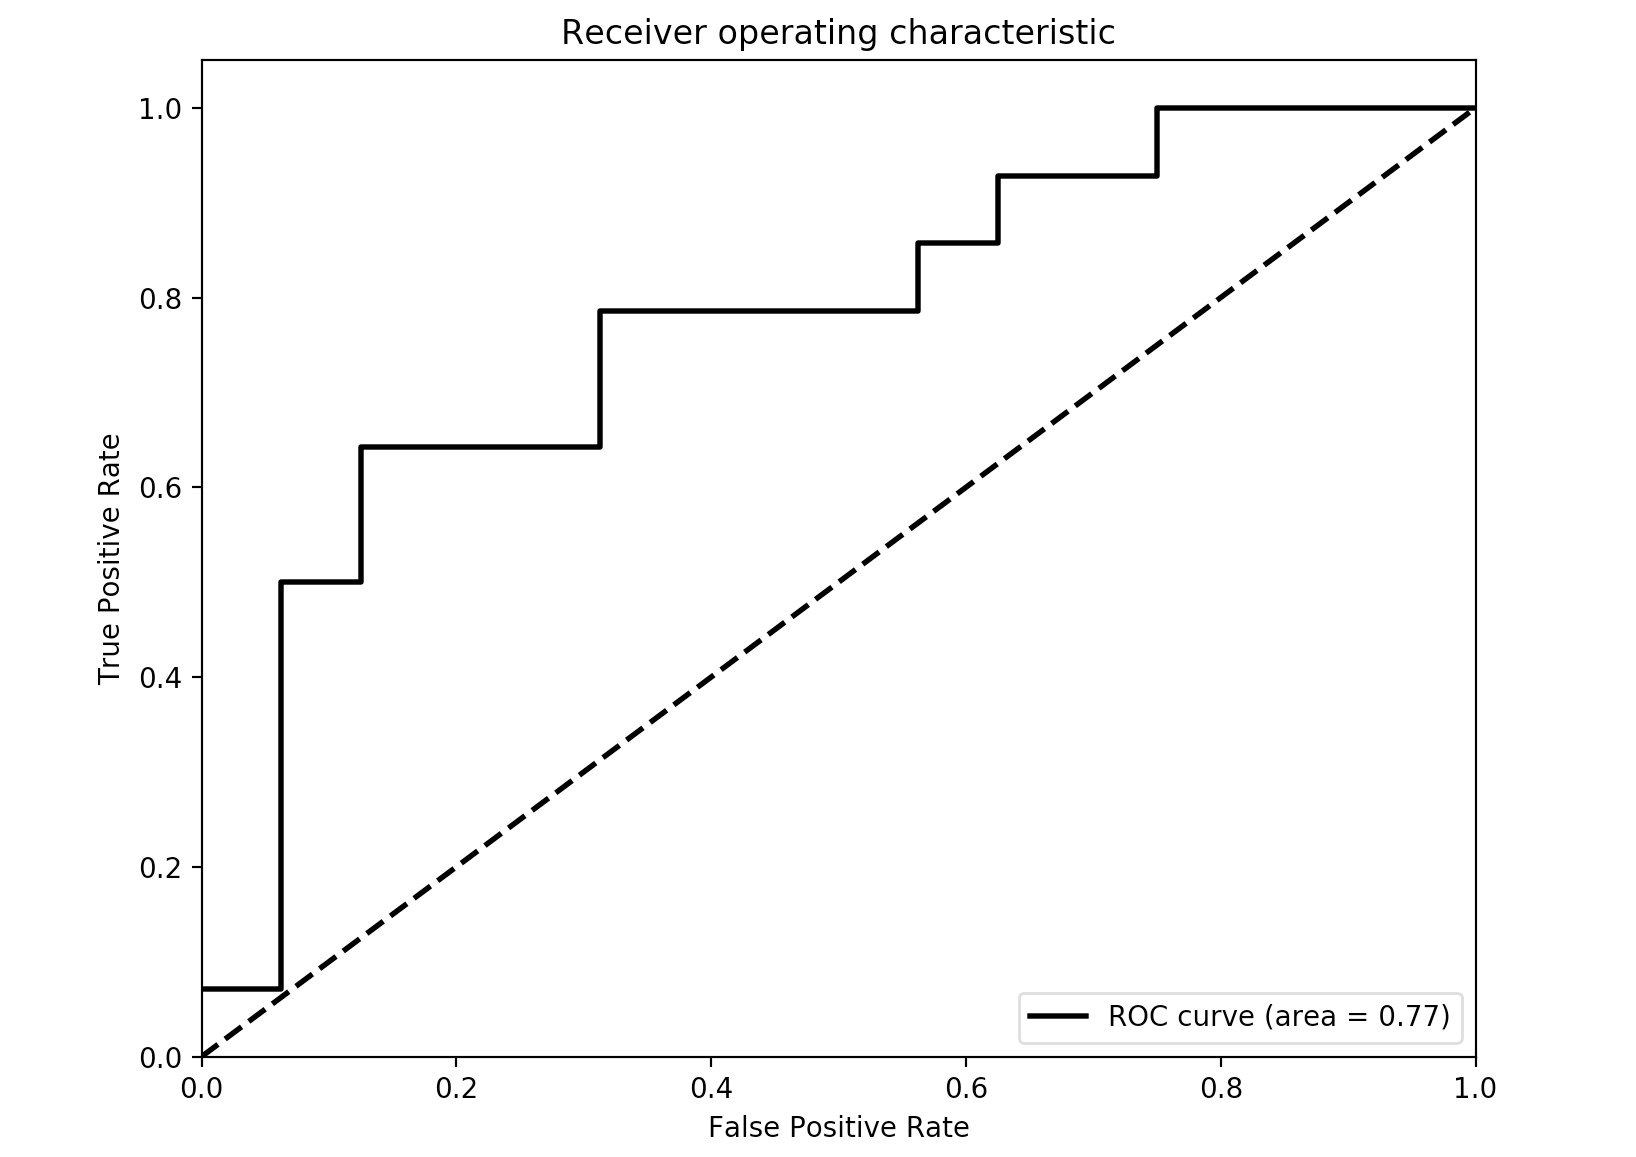
\includegraphics[scale=0.33]{./imagenes/roc}
\end{figure}
\end{frame}

\begin{frame}{Media geométrica.}
\begin{center}
	$g = \sqrt{a^+ \cdot a^-}$
\end{center}

donde a$^+$ denota la precisión en las instancias positivas —esto es \textit{TPR}— y a$^-$ denota la precisión en las instancias positivas —esto es \textit{TNR}—, y se calcula de la siguiente forma:

\begin{equation}
	TNR = \frac{TP}{TP + FN}
\end{equation}
\end{frame}

\begin{frame}{Porcentaje de acierto.}
	\centering
	\begin{tikzpicture}
	\draw[xstep=2cm,ystep=1,color=gray] (0, 0) grid (10, 1);
	\node at (1,0.5) {1};
	\node at (3,0.5) {0};
	\node at (5,0.5) {1};
	\node at (7,0.5) {1};
	\node at (9,0.5) {0};
	\end{tikzpicture}
	
	\begin{tikzpicture}
	\draw[xstep=2cm,ystep=1,color=gray] (0, 0) grid (10, 1);
	\node at (1,0.5) {1};
	\node at (3,0.5) {1};
	\node at (5,0.5) {0};
	\node at (7,0.5) {1};
	\node at (9,0.5) {0};
	\end{tikzpicture}
	
	\begin{tikzpicture}
	\draw[xstep=2cm,ystep=1,opacity=0] (0, 0) grid (10, 1);
	\node at (1,0.5) {\cmark};
	\node at (3,0.5) {\xmark};
	\node at (5,0.5) {\xmark};
	\node at (7,0.5) {\cmark};
	\node at (9,0.5) {\cmark};
	\end{tikzpicture}
	
	60\%
\end{frame}


\begin{frame}{ecoli3.}
\centering
\scalebox{0.78}{\begin{tabular}{l|cccccc}
\textbf{Algoritmo} & \multicolumn{1}{c}{\textbf{j48auc}} & \multicolumn{1}{c}{\textbf{j48gm}} & \multicolumn{1}{c}{\textbf{j48\_\%}} & \multicolumn{1}{c}{\textbf{SVMauc}} & \multicolumn{1}{c}{\textbf{SVMgm}} & \multicolumn{1}{c}{\textbf{SVM\_\%}} \\
\midrule
\textbf{BC} & \cellcolor[rgb]{ .871,  .906,  .957}0.768 & \cellcolor[rgb]{ .976,  .98,  .996}0.751 & \cellcolor[rgb]{ .918,  .937,  .973}79.485 & \cellcolor[rgb]{ .976,  .459,  .467}0.87 & \cellcolor[rgb]{ .976,  .439,  .447}0.866 & \cellcolor[rgb]{ .98,  .98,  .996}81.287 \\
\textbf{CNN} & \cellcolor[rgb]{ .533,  .667,  .839}0.653 & \cellcolor[rgb]{ .541,  .671,  .839}0.512 & \cellcolor[rgb]{ .976,  .506,  .514}91.085 & \cellcolor[rgb]{ .353,  .541,  .776}0.5 & \cellcolor[rgb]{ .353,  .541,  .776}0 & \cellcolor[rgb]{ .98,  .557,  .569}89.577 \\
\textbf{CPM} & \cellcolor[rgb]{ .545,  .675,  .843}0.657 & \cellcolor[rgb]{ .557,  .686,  .847}0.522 & \cellcolor[rgb]{ .627,  .733,  .871}64.007 & \cellcolor[rgb]{ .533,  .667,  .839}0.557 & \cellcolor[rgb]{ .651,  .749,  .878}0.274 & \cellcolor[rgb]{ .98,  .624,  .631}88.401 \\
\textbf{ClusterOSS} & \cellcolor[rgb]{ .988,  .988,  1}0.807 & \cellcolor[rgb]{ .988,  .988,  1}0.757 & \cellcolor[rgb]{ .824,  .871,  .941}74.522 & \cellcolor[rgb]{ .984,  .729,  .737}0.782 & \cellcolor[rgb]{ .984,  .804,  .812}0.678 & \cellcolor[rgb]{ .98,  .98,  .996}81.232 \\
\textbf{EE} & \cellcolor[rgb]{ .98,  .604,  .612}0.875 & \cellcolor[rgb]{ .973,  .412,  .42}0.858 & \cellcolor[rgb]{ .961,  .969,  .988}81.985 & \cellcolor[rgb]{ .976,  .459,  .467}0.869 & \cellcolor[rgb]{ .976,  .439,  .447}0.866 & \cellcolor[rgb]{ .976,  .98,  .996}81.121 \\
\textbf{ENN} & \cellcolor[rgb]{ .988,  .898,  .91}0.823 & \cellcolor[rgb]{ .988,  .945,  .957}0.765 & \cellcolor[rgb]{ .976,  .416,  .424}92.5 & \cellcolor[rgb]{ .871,  .906,  .957}0.661 & \cellcolor[rgb]{ .969,  .973,  .992}0.565 & \cellcolor[rgb]{ .976,  .463,  .471}91.36 \\
\textbf{EUS} & \cellcolor[rgb]{ .984,  .8,  .812}0.84 & \cellcolor[rgb]{ .976,  .541,  .549}0.836 & \cellcolor[rgb]{ .988,  .988,  1}83.272 & \cellcolor[rgb]{ .973,  .412,  .42}0.884 & \cellcolor[rgb]{ .973,  .412,  .42}0.879 & \cellcolor[rgb]{ .988,  .988,  1}81.544 \\
\textbf{IHTS} & \cellcolor[rgb]{ .353,  .541,  .776}0.591 & \cellcolor[rgb]{ .353,  .541,  .776}0.408 & \cellcolor[rgb]{ .353,  .541,  .776}49.118 & \cellcolor[rgb]{ .988,  .988,  1}0.697 & \cellcolor[rgb]{ .894,  .922,  .965}0.495 & \cellcolor[rgb]{ .353,  .541,  .776}54.706 \\
\textbf{IPADE-ID} & \cellcolor[rgb]{ .973,  .412,  .42}0.908 & \cellcolor[rgb]{ .976,  .42,  .427}0.857 & \cellcolor[rgb]{ .984,  .722,  .729}87.61 & \cellcolor[rgb]{ .988,  .933,  .945}0.715 & \cellcolor[rgb]{ .988,  .988,  1}0.581 & \cellcolor[rgb]{ .749,  .82,  .914}71.581 \\
\textbf{NCL} & \cellcolor[rgb]{ .976,  .976,  .992}0.803 & \cellcolor[rgb]{ .91,  .933,  .973}0.715 & \cellcolor[rgb]{ .973,  .412,  .42}92.555 & \cellcolor[rgb]{ .396,  .573,  .792}0.514 & \cellcolor[rgb]{ .435,  .596,  .804}0.076 & \cellcolor[rgb]{ .976,  .541,  .553}89.871 \\
\textbf{NM} & \cellcolor[rgb]{ .69,  .776,  .894}0.706 & \cellcolor[rgb]{ .718,  .796,  .902}0.61 & \cellcolor[rgb]{ .831,  .875,  .941}74.853 & \cellcolor[rgb]{ .812,  .863,  .937}0.643 & \cellcolor[rgb]{ .988,  .882,  .894}0.636 & \cellcolor[rgb]{ .443,  .604,  .808}58.658 \\
\textbf{OSS} & \cellcolor[rgb]{ .965,  .973,  .992}0.8 & \cellcolor[rgb]{ .894,  .922,  .965}0.707 & \cellcolor[rgb]{ .976,  .486,  .494}91.415 & \cellcolor[rgb]{ .38,  .561,  .784}0.509 & \cellcolor[rgb]{ .431,  .596,  .804}0.074 & \cellcolor[rgb]{ .98,  .592,  .6}88.989 \\
\textbf{RU} & \cellcolor[rgb]{ .988,  .898,  .91}0.823 & \cellcolor[rgb]{ .98,  .682,  .69}0.811 & \cellcolor[rgb]{ .937,  .953,  .98}80.68 & \cellcolor[rgb]{ .976,  .478,  .486}0.863 & \cellcolor[rgb]{ .976,  .455,  .463}0.858 & \cellcolor[rgb]{ .953,  .961,  .984}80.074 \\
\textbf{SCB} & \cellcolor[rgb]{ .98,  .675,  .686}0.862 & \cellcolor[rgb]{ .988,  .871,  .882}0.778 & \cellcolor[rgb]{ .98,  .576,  .588}89.908 & \cellcolor[rgb]{ .98,  .616,  .627}0.818 & \cellcolor[rgb]{ .976,  .557,  .565}0.805 & \cellcolor[rgb]{ .973,  .412,  .42}92.279 \\
\textbf{TL} & \cellcolor[rgb]{ .988,  .918,  .925}0.82 & \cellcolor[rgb]{ .988,  .922,  .933}0.769 & \cellcolor[rgb]{ .976,  .451,  .459}91.985 & \cellcolor[rgb]{ .353,  .541,  .776}0.5 & \cellcolor[rgb]{ .353,  .541,  .776}0 & \cellcolor[rgb]{ .98,  .557,  .569}89.577 \\
\midrule
\textbf{original} & \textbf{0.805} & \textbf{0.753} & \textbf{93.438} & \textbf{0.5} & \textbf{0} & \textbf{89.577} \\
\end{tabular}}
\end{frame}

\begin{frame}{Nube de puntos.}
\begin{figure}[H]
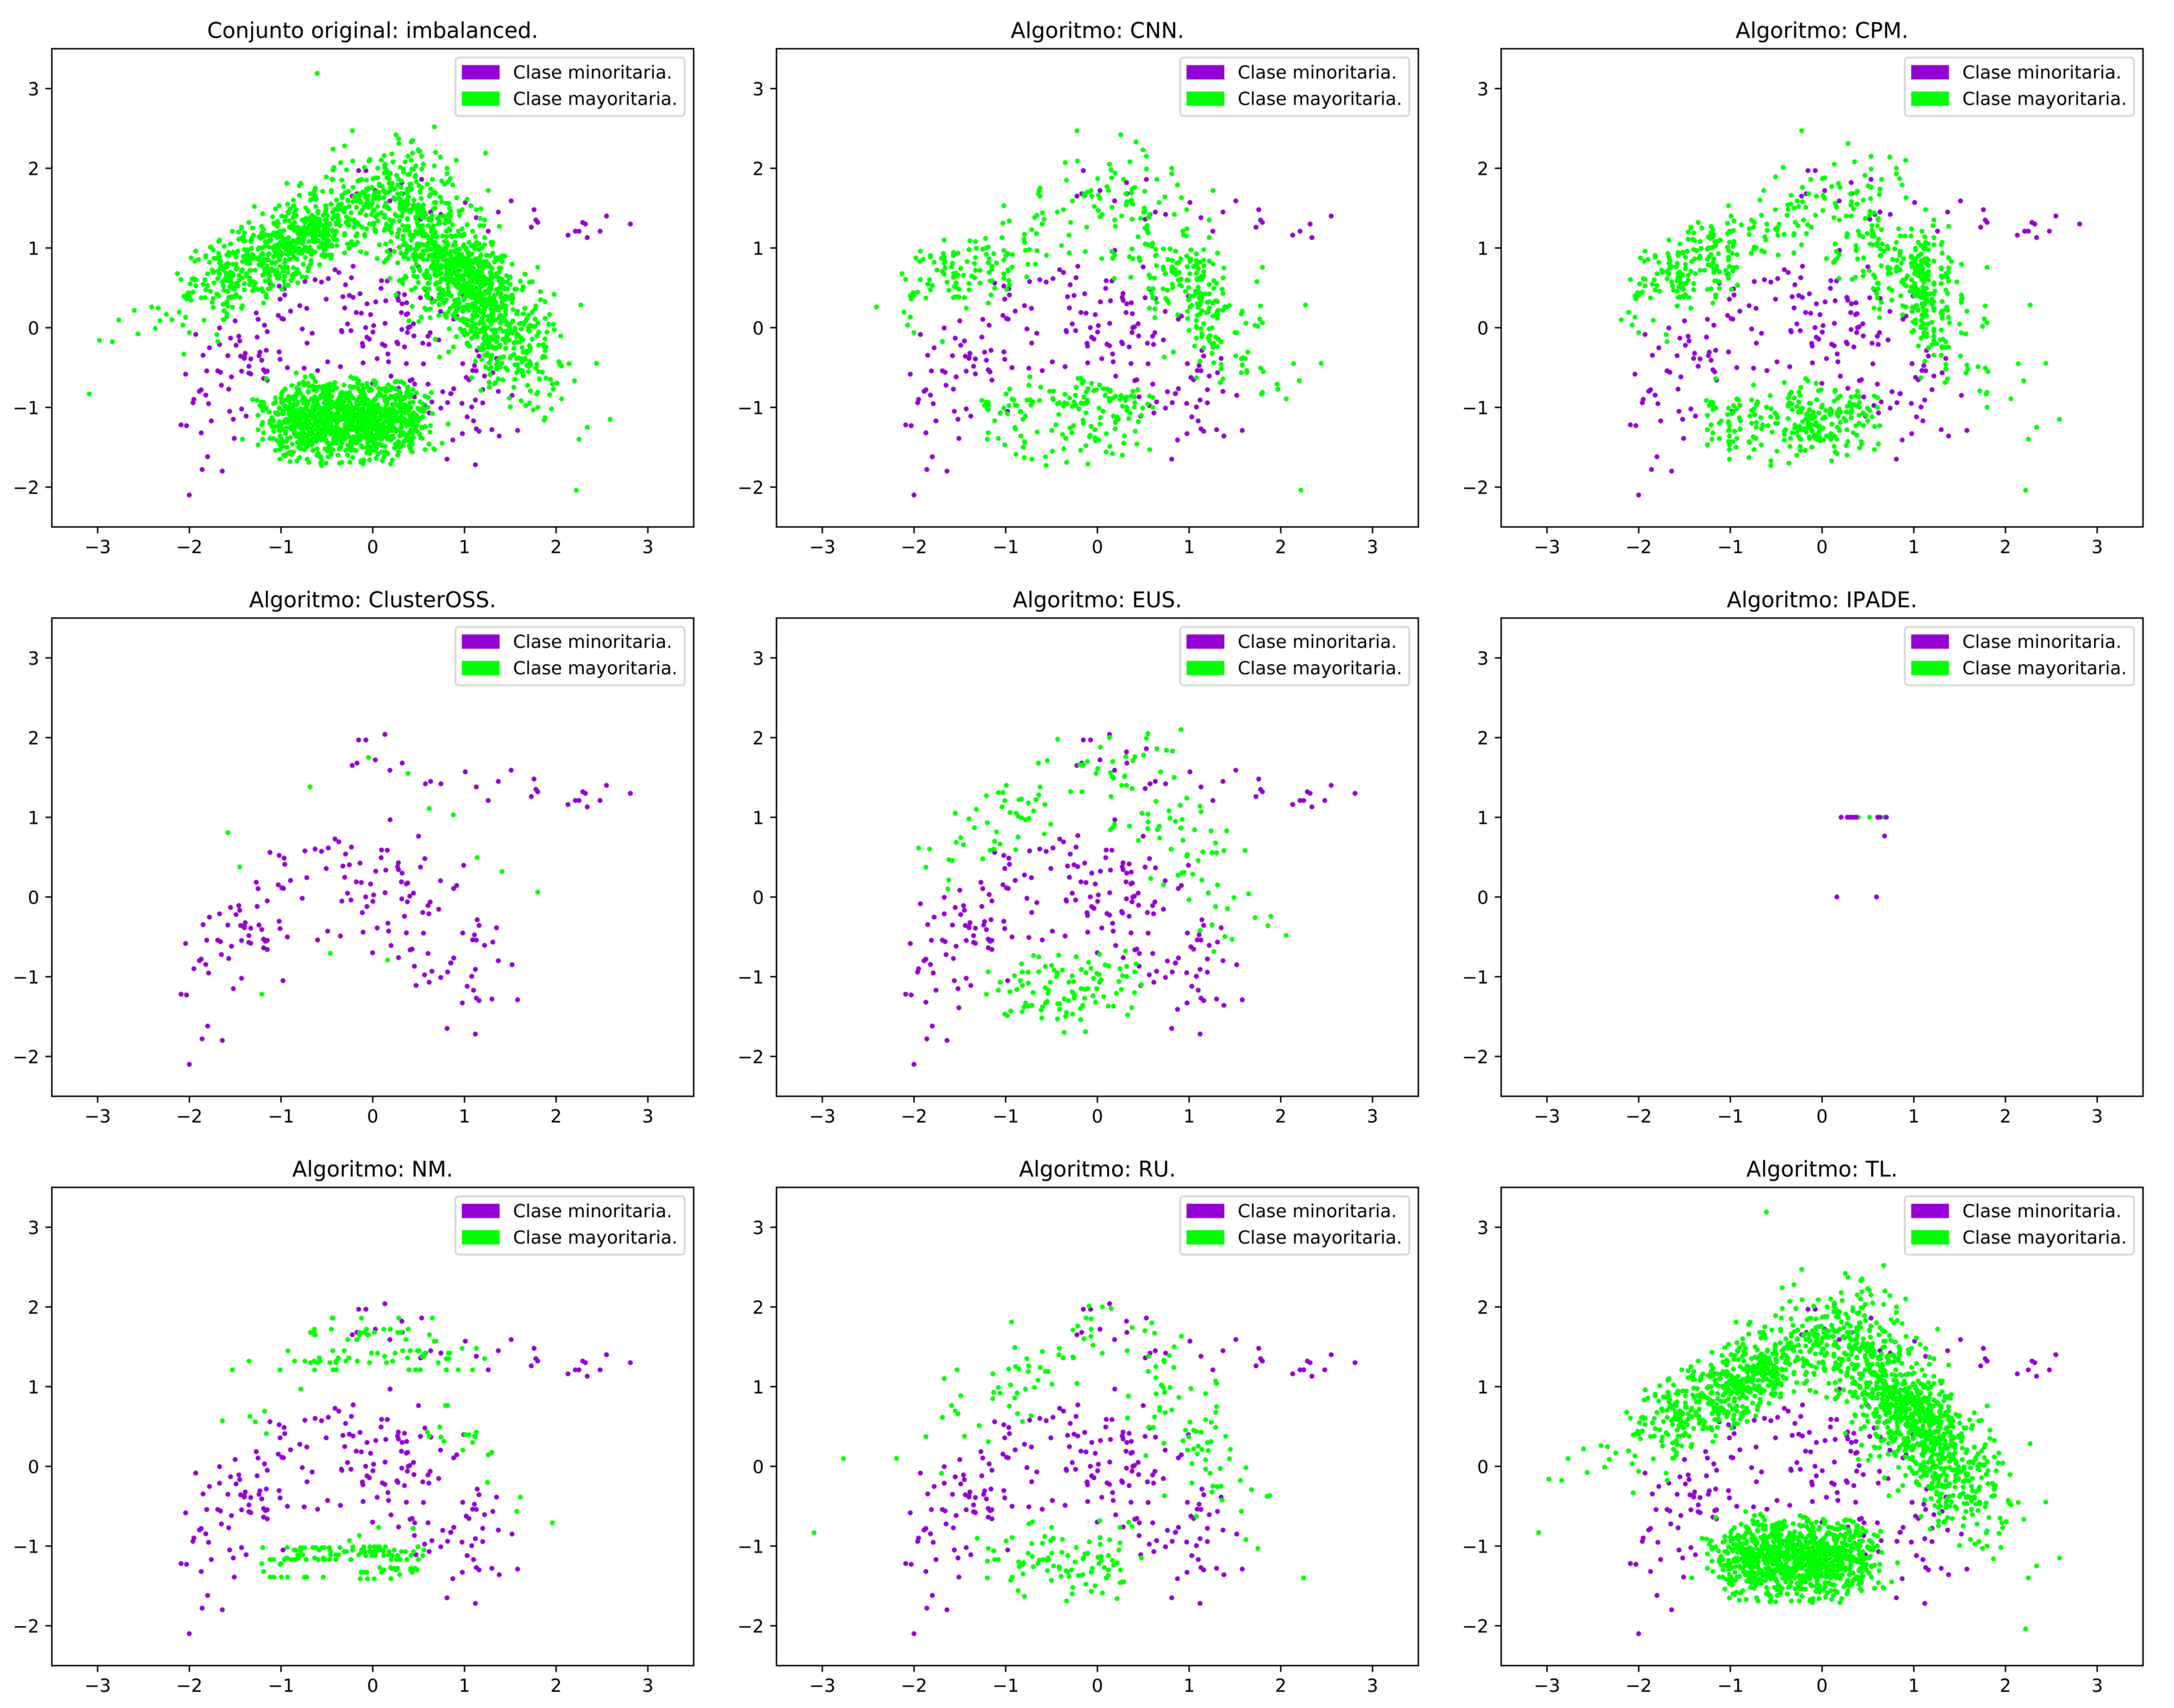
\includegraphics[scale=0.065]{./imagenes/np}
\end{figure}
\end{frame}

\section{Trabajos futuros.}

\begin{frame}{Trabajos futuros.}
\begin{figure}[H]
\centering

\includegraphics[scale=0.17]{./imagenes/spark_gpu}
\end{figure}
\end{frame}

\begin{frame}[allowframebreaks]{References.}
	\bibliography{bibliografia}
	\bibliographystyle{abbrv}
\end{frame}

\begin{frame}[standout]
  Gracias.
\end{frame}

\end{document}